\chapter{SİN\texorpdfstring{\textsuperscript{3}}{3} TABANLI İLERİ BESLEME KOMPANZASYONU VE KAPALI ÇEVRİM ANALİZİ}
\label{chap:sin3}

Bölüm~\ref{chap:anahtarlama}, nötr anahtar susturma yönteminin ters akım dolaşımını keserek düşük güç verimini artırdığını, karşılığında akımı süreksiz iletime zorlayıp özellikle üçüncü harmoniği büyüttüğünü göstermiştir: yaklaşık \SI{2.3}{\ampere} faz akımında şebeke akımı THD'si deneyde \%15'ten \%47'ye, kalibre benzetimde \%39,5'ten \%56,7'ye çıkmaktadır (Tablo~\ref{tab:kalibrasyon-karsilastirma}). Bölüm~\ref{chap:sin3}, harmonik cezayı azaltmak için tezin ikinci katkısı olan Sin\textsuperscript{3} tabanlı ileri besleme kompanzasyonunu ele almaktadır; susturma ile birlikte kullanılan terim, deneyde THD'yi \%14'e, yani klasik anahtarlama düzeyine indirmektedir (Alt Bölüm~\ref{sec:kalibrasyon}). Bölümün amacı, THD iyileşmesinin arkasındaki matematiksel yapıyı kurmak; Sin\textsuperscript{3} teriminin benzetim modelindeki biçimini ve kompanzasyon katsayılarını doğru trigonometrik özdeşlikle vermek; ardından akım geri beslemeli Senaryo~4 (S4) modelinde düşük, orta ve anma akımında kapalı çevrim başarımını ve kararlılığı göstermektir. Sin\textsuperscript{3} teriminin bir denetleyici değil, modülasyon toplamına çevrim dışından eklenen bir ileri besleme girişi olduğu ve kararlılık marjlarını değiştirmediği Alt Bölüm~\ref{sec:kararlilik-bode} içinde analitik, frekans alanı ve zaman alanı kanıtlarıyla gösterilmektedir.

\section{Sin\texorpdfstring{\textsuperscript{3}}{3} Bileşeninin Matematiksel Tanımı}

Zaman $t$, şebeke temel açısal frekansı $\omega_0$, PLL faz başlangıcı $\phi$ ve boyutsuz elektriksel açı $\theta=\omega_0t+\phi$ ile gösterilsin. Kullanılan trigonometrik özdeşlik
\begin{equation}
  \sin^3\theta=\frac{3}{4}\sin\theta-\frac{1}{4}\sin(3\theta)
  \label{eq:sin3-acilimi}
\end{equation}
biçimindedir. Eşitlik~\eqref{eq:sin3-acilimi} uyarınca $\sin^3\theta$ terimi yalnız üçüncü harmonikten oluşmaz; temel bileşen ile ters işaretli üçüncü harmonik bileşenini sabit bir oranla birlikte taşır. Boyutsuz Sin\textsuperscript{3} ileri besleme komutu $u_{\mathrm{ff},\sin^3}(\theta)$, temel bileşen katsayısı $D_1$ ve küp teriminin katsayısı $D_3$ ile
\begin{equation}
  u_{\mathrm{ff},\sin^3}(\theta)=D_1\sin\theta+D_3\sin^3\theta
  \label{eq:sin3-genel-komut}
\end{equation}
olarak tanımlandığında Eşitlik~\eqref{eq:sin3-acilimi} kullanılarak
\begin{equation}
  u_{\mathrm{ff},\sin^3}(\theta)
  =\left(D_1+\frac{3D_3}{4}\right)\sin\theta-\frac{D_3}{4}\sin(3\theta)
  \label{eq:sin3-esdeger-katsayilar}
\end{equation}
elde edilir. Eşitlik~\eqref{eq:sin3-esdeger-katsayilar} içinde $D_1+3D_3/4$ temel sinüs katsayısını, $-D_3/4$ ise doğrudan üçüncü harmonik katsayısını gösterir; tezde iki ifade, katsayı çiftinin harmonik eşdeğeri olarak anılır ve ayrı bir simgeyle gösterilmez. Doğrudan $\sin(3\theta)$ enjeksiyonu ile $\sin^3\theta$ terimi aynı işlem değildir: aynı sayısal $D_3$ değeri iki gösterimde farklı temel ve üçüncü harmonik genliği üretir.

Uygulamanın yürütülebilir tanımı Simulink benzetim modelleridir; gösterim, modelin blok yapısından okunmuştur. Senaryo~3 (S3) modelinde birim genlikli sinüs işaretinin küpü alınmakta ve küp terimi katsayısıyla çarpılarak temel bileşen terimine eklenmektedir; terim pozitif işaretlidir, ek bir normalizasyon içermez ve modelde $\sin(3\theta)$ üreten blok bulunmamaktadır. Toplam, görev oranı komutuna açık çevrim ileri besleme olarak girer. Parametre dosyasındaki ilk değerlerle ($D_1=0{,}45$, $D_3=0{,}39$) Eşitlik~\eqref{eq:sin3-esdeger-katsayilar} $u_{\mathrm{ff},\sin^3}(\theta)=0{,}7425\sin\theta-0{,}0975\sin3\theta$ verir ve komutun tepe değeri $D_1+D_3=0{,}84$'tür. Alt Bölüm~\ref{sec:kalibrasyon} içinde deney özetine kalibre edilen S3 katsayılarıyla (Tablo~\ref{tab:sistem-parametreleri}) harmonik eşdeğer $D_1+3D_3/4=0{,}7317$ ve $-D_3/4=-0{,}0961$ olur.

Tezde görev oranı komutunun sinüs ve küp terimi katsayıları tek adla, $(D_1,D_3)$ çiftiyle gösterilmektedir. $D_3=0$ özel durumunda $D_1$, sinüzoidal görev oranının tepe katsayısı $d_m$'ye eşittir. Anahtarlamalı benzetim modelinde aynı katsayıların $x$ numaralı senaryodaki değerleri $K_{1x}$ ve $K_{3x}$ parametreleriyle taşınır (örneğin S4 için $K_{14}$ ve $K_{34}$); S3 ve S4 değerleri kalibre değerlerdir. Alt Bölüm~\ref{sec:sin3-yeniden-tarama} içindeki tek endüktanslı analitik modelden çıkan $(D_1,D_3)$ değerleri ise aday niteliğindedir; analitik aday ile kalibre model değeri farklı model katmanlarına aittir ve birbirinin yerine kullanılmamaktadır.

\section{Basitleştirilmiş Türetimlerin Geçerlilik Sınırı}

Kompanzasyon katsayılarının tek bir cebirsel iptal koşulundan, örneğin sabit bir $D_1/D_3$ oranından türetilmesi anahtarlamalı dönüştürücüde geçerli değildir. Birinci gerekçe, belirli bir çalışma noktasında gözlenen temel ve üçüncü harmonik genliklerinin oranının girişten bağımsız bir sistem aktarım fonksiyonu olmamasıdır; oran yalnız o dalga biçimini ve o çalışma noktasını tarif eder. İkinci gerekçe, anahtarlamalı, doğrusal olmayan ya da periyodik zamanla değişen bir sistemde süperpozisyonun kanıtlanmadan uygulanamamasıdır; giriş dalga biçimi değiştiğinde aynı skaler oranın yeniden kullanılması örtük bir doğrusallık varsayımıdır. Üçüncü gerekçe, komutun frekans içeriği ile dönüştürücünün çıkış akımının aynı büyüklük olmamasıdır; çıkıştaki harmonik iptal koşulu, denetlenen sistemin dinamiği ve harmonikler arası bağlaşım bilinmeden yalnız trigonometrik özdeşlikten çıkarılamaz.

Periyodik zamanla değişen sistemin genel çerçevesi harmonik aktarım fonksiyonudur (harmonic transfer function, HTF). Kesilmiş harmonik giriş ve çıkış vektörleri $\mathbf{U}(s)$ ile $\mathbf{I}(s)$, harmonik aktarım matrisi $\mathbf{G}_{\mathrm{H}}(s)$, matrisin $(k,n)$ elemanı $G_{k,n}(s)$ ve kesme mertebesi $N_h$ ile gösterildiğinde
\begin{equation}
  \mathbf{I}(s)=\mathbf{G}_{\mathrm{H}}(s)\mathbf{U}(s),
  \qquad
  I_k(s)=\sum_{n=-N_h}^{N_h}G_{k,n}(s)U_n(s)
  \label{eq:htf-matris-iliskisi}
\end{equation}
yazılır \citep{Wereley1991,Liao2022}. Eşitlik~\eqref{eq:htf-matris-iliskisi}, tek bir giriş harmoniğinin birden fazla çıkış harmoniğine bağlaşabileceğini gösterir. Geçerli bir HTF modeli için çalışma noktası, frekans taraması, $N_h$ ve kesme hatası birlikte belirtilmelidir. Kompanzasyon katsayıları HTF çerçevesinde ya periyodik çalışma noktası çevresinde doğrusallaştırılmış model üzerinden ya da küçük işaretli harmonik enjeksiyon ölçümleriyle belirlenmelidir; katsayıların çalışma noktasına bağlılığı Alt Bölüm~\ref{sec:sin3-yeniden-tarama} içinde sayısal olarak gösterilmektedir.

Tezde temel--üçüncü harmonik bağlaşımı, anma akımı çalışma noktasında anahtarlamalı S4 modeli üzerinden doğrudan ölçülmüştür. $K_{34}$ açık ve kapalı iki benzetim arasındaki $L_1$ akımı farkı, Sin\textsuperscript{3} girişinin akıma katkısını verir. Anahtarlamalı modelde fark temel bileşende \SI{4.44}{\ampere} RMS, $\angle-43{,}4^{\circ}$; üçüncü harmonikte \SI{2.32}{\ampere} RMS, $\angle110{,}4^{\circ}$'dir. Doğrusal zamanla değişmeyen ortalama model aynı farkı \SI{4.51}{\ampere}, $\angle-40{,}7^{\circ}$ ve \SI{2.23}{\ampere}, $\angle102{,}9^{\circ}$ olarak öngörmektedir. Ortalama modelde çapraz harmonik terimi bulunmadığından, \SI{25}{\ampere} noktasında Eşitlik~\eqref{eq:htf-matris-iliskisi} matrisinin köşegen dışı katkısı en çok temel bileşende \%1,5 ve $2{,}7^{\circ}$, üçüncü harmonikte \%3,8 ve $7{,}5^{\circ}$ düzeyindedir. Düşük akımda süreksiz iletim köprünün etkin kazancını frekansla değiştirdiğinden (Alt Bölüm~\ref{sec:kararlilik-bode}) aynı sonuç \SI{2.3}{\ampere} noktasına genellenmemektedir.

Kompanzasyonun hedefi, akımın üçüncü harmonik fazına ters yönde bir modülasyon bileşeni üretirken temel akım genliğini korumaktır. Uygulama kazancı yalnız THD eniyilemesiyle seçilmemeli; modülasyon doygunluğu, DA bara kullanımı, akım RMS değeri, denetim eforu ve düşük güçten orta güce geçişte süreklilik koşulları birlikte değerlendirilmelidir. Üçüncü harmonik enjeksiyonunun modülasyon kullanımını değiştirebildiği bilinmektedir; tezdeki amaç ise klasik üçüncü harmonik PWM ile DA bara kullanımını artırmak değil, nötr susturmanın oluşturduğu akım zarfı bozulmasını azaltmaktır \citep{Holmes2003}.

\section{Düşük Güçte Harmonik Oluşum Mekanizması}
\label{sec:harmonik-mekanizma}

Şekil~\ref{fig:susturma-esdeger} altında verilen senkron olmayan iki alçaltıcı eşdeğeri, pozitif ve negatif alternansların aynı fiziksel mekanizmayla incelenmesini sağlar. Pozitif alternansta etkin yarım bara gerilimi $V_h$, anlık şebeke gerilimi $v_g(\theta)>0$, anahtarlama periyodu $T_s$, boyutsuz görev oranı $d(\theta)\in[0,1]$ ve eşdeğer endüktans $L$ olarak tanımlansın. İdeal anahtarlama periyodu modeli ve periyot boyunca yaklaşık sabit gerilim kabulü altında anahtar iletim süresindeki akım tepe değeri $I_{\mathrm{pk}}(\theta)$
\begin{equation}
  I_{\mathrm{pk}}(\theta)=\frac{V_h-v_g(\theta)}{L}\,d(\theta)T_s
  \label{eq:dcm-tepe-akimi}
\end{equation}
olur. Eşitlik~\eqref{eq:dcm-tepe-akimi}, iletim başlangıcında akımın sıfır olduğu süreksiz iletim (discontinuous conduction mode, DCM) darbesi içindir. Anahtar kesime girdiğinde akım $-v_g/L$ eğimiyle sıfıra düşerse, boşalma süresinin $T_s$'ye oranı olan boyutsuz $\delta(\theta)$
\begin{equation}
  \delta(\theta)=\left(\frac{V_h}{v_g(\theta)}-1\right)d(\theta)
  \label{eq:dcm-bosalma-suresi}
\end{equation}
olarak bulunur. Eşitlik~\eqref{eq:dcm-bosalma-suresi}, yalnızca $v_g(\theta)>0$ ve akımın aynı periyotta sıfıra ulaştığı aralıkta geçerlidir. Üçgensel akım darbesinin bir anahtarlama periyodundaki ortalaması $\bar i_L(\theta)$
\begin{equation}
  \bar i_L(\theta)=\frac{1}{2}I_{\mathrm{pk}}(\theta)\,[d(\theta)+\delta(\theta)]
  =\frac{T_sV_h}{2L}\frac{V_h-v_g(\theta)}{v_g(\theta)}d^2(\theta)
  \label{eq:dcm-ortalama-akim}
\end{equation}
ifadesini verir \citep{Erickson2001,Chen2010}. Eşitlik~\eqref{eq:dcm-ortalama-akim}, Eşitlik~\eqref{eq:dcm-tepe-akimi} ile Eşitlik~\eqref{eq:dcm-bosalma-suresi} kullanılarak üçgen alanından elde edilmiştir. Sinüzoidal görev oranının tepe katsayısı $d_m$ ve şebeke geriliminin tepe değeri $V_m$ olmak üzere $d(\theta)=d_m\sin\theta$ ve $v_g(\theta)=V_m\sin\theta$ kabulü altında pozitif alternans zarfı
\begin{equation}
  \bar i_L(\theta)=\frac{T_sV_hd_m^2}{2LV_m}\sin\theta\,[V_h-V_m\sin\theta],
  \qquad 0<\theta<\pi
  \label{eq:dcm-sinus-zarfi}
\end{equation}
biçimine dönüşür. Eşitlik~\eqref{eq:dcm-sinus-zarfi}, görev oranı sinüzoidal olsa bile ortalama akımın saf sinüs kalmadığını doğrudan göstermektedir: zarf, $\sin\theta$ ile $[V_h-V_m\sin\theta]$ çarpımından oluştuğu için sıfır geçişlerinde sinüsten hızlı yükselir ve alternans ortasında çöker. Düşük güçte çalışma noktasına bağlı akım harmoniklerinin büyüyebildiği, saha ölçümü ile zamanla değişen modeller üzerinden de raporlanmıştır \citep{Chicco2009,Du2013}.

Mekanizma, kalibre S2 çalışma noktasında Şekil~\ref{fig:harmonik-mekanizma} üzerinde adım adım gösterilmiştir. Şekilde $V_{\mathrm{dc}}=\SI{395}{\volt}$, $V_m=\SI{171.1}{\volt}$, $L=L_1=\SI{600}{\micro\henry}$ ve $f_s=\SI{10}{\kilo\hertz}$ kullanılmıştır (Tablo~\ref{tab:sistem-parametreleri}). $d_m$, Eşitlik~\eqref{eq:dcm-ccm-parcali-model} ile kurulan parçalı modelin $L_1$ temel bileşeni kalibre S2 benzetimindeki $L_1$ temel bileşenine (\SI{2.10}{\ampere} RMS) eşitlenerek $0{,}768$ bulunmuştur; değer, kalibre S2 modelinin modülasyon genlik ölçeğiyle ($K_{12}=0{,}768$, Alt Bölüm~\ref{sec:kalibrasyon}) aynıdır. Görev oranı alternans boyunca kritik görev oranının altında kaldığından faz kolu yarım periyodun tamamında süreksiz iletimdedir (Şekil~\ref{fig:harmonik-mekanizma}a). Akımı yükselten $V_h-v_g$ gerilim payı alternans ortasında en küçük değerine iner (b); görev oranı en büyük olduğu halde tepe akım alternans ortasında çöker ve en büyük değerlerine yaklaşık \SI{2}{\milli\second} ve \SI{8}{\milli\second} çevresinde ulaşır (c). Ortalama akım zarfı iki tepeli bir biçim alır; üçüncü harmoniğin temel bileşene oranı parçalı modelde \%55,6, kalibre benzetimde \%55,9'dur (d). Oran Tablo~\ref{tab:dcm-saf-sinus-harmonikleri} içindeki \%39,96'dan büyüktür: zarfın biçimi $d_m$'den bağımsız olsa da $V_m/V_h$ oranına bağlıdır ve oran S1 noktasında $0{,}785$, S2 noktasında $0{,}866$'dır. Benzetim zarfındaki iki tepe arasındaki asimetri, analitik modelde bulunmayan $C_f$--$L_2$ dinamiği ve akımın şebeke gerilimine göre fazı ile ilişkilendirilebilir. Anlık akımda üçgen darbeler her anahtarlama periyodunda sıfıra iner ve ters yöne geçmez (e); susturmanın verim kazancı ile harmonik cezası aynı darbe biçiminden doğmaktadır.

\begin{figure}[H]
  \centering
  \includegraphics[width=0.94\textwidth]{sin3/harmonik_olusum_mekanizmasi.pdf}
  \caption[Susturmalı faz kolunda üçüncü harmonik oluşum mekanizması]{Susturmalı faz kolunda üçüncü harmonik oluşum mekanizması, kalibre S2 çalışma noktası, pozitif alternans: (a) sinüzoidal görev oranı ve süreksiz iletim sınırı, (b) iletimde endüktör gerilimi, (c) anahtarlama periyodu tepe akımı, (d) anahtarlama periyodu ortalama akımı, (e) anlık endüktör akımı. Analitik eğriler Eşitlik~\eqref{eq:dcm-tepe-akimi}--\eqref{eq:dcm-ccm-parcali-model} ile, gri eğriler kalibre S2 benzetim kaydından (son tam şebeke periyodu) elde edilmiştir.}
  \label{fig:harmonik-mekanizma}
\end{figure}

DCM koşulu darbenin aynı anahtarlama periyodunda sona ermesini gerektirir:
\begin{equation}
  d(\theta)+\delta(\theta)\leq 1
  \quad\Longrightarrow\quad
  d(\theta)\leq d_{\mathrm{krit}}(\theta)=\frac{v_g(\theta)}{V_h}.
  \label{eq:dcm-kritik-gorev}
\end{equation}
Eşitlik~\eqref{eq:dcm-kritik-gorev} içindeki kritik görev oranı faz açısına ve gerilim oranına bağlıdır; tek bir evrensel sayı değildir. Senaryo~1 (S1) çalışma noktasının DA bara ve şebeke gerilimleriyle (Tablo~\ref{tab:sistem-parametreleri}) kritik görev oranının tepe değeri $V_m/V_h\simeq0{,}785$'tir ve Alt Bölüm~\ref{sec:sin3-yeniden-tarama} içindeki sayısal tarama, $d_m$ sınırı aştığında alternans ortasında sürekli iletime (continuous conduction mode, CCM) geçildiğini doğrulamaktadır. Sıfır geçişte $v_g\rightarrow0$ olduğundan ideal ifadenin tek başına kullanılması uygun değildir; ölü zaman, en küçük darbe süresi ve sonlu akım eşiği ayrıca uygulanmalıdır.

DCM zarfı ile sürekli iletim modeli ortak bir görev oranı üzerinden birleştirilebilir. Analitik modelde görev oranı, Eşitlik~\eqref{eq:sin3-genel-komut} ile aynı $(D_1,D_3)$ katsayılarıyla
\begin{equation}
  d(\theta)=D_1\sin\theta+D_3\sin^3\theta
  \label{eq:ccm-gorev-harmonik}
\end{equation}
yazılsın. Analitik modelden bulunan $(D_1,D_3)$ değerleri tek endüktanslı kayıpsız modele aittir ve benzetim modelindeki $K_{1x}$, $K_{3x}$ değerlerine bire bir eşit değildir. Pozitif alternansta kayıpsız CCM ortalama diferansiyel denklemi
\begin{equation}
  L\frac{\mathrm{d}\bar i_{L,\mathrm{CCM}}}{\mathrm{d}t}
  =V_h d(\theta)-V_m\sin\theta
  \label{eq:ccm-diferansiyel}
\end{equation}
biçimindedir \citep{Erickson2001,Mohan2003}. Eşitlik~\eqref{eq:ccm-diferansiyel}, $\theta=\omega_0t+\phi$ bağı ve Eşitlik~\eqref{eq:ccm-gorev-harmonik} kullanılarak integre edildiğinde
\begin{equation}
  \bar i_{L,\mathrm{CCM}}(\theta)
  = I_0+\frac{V_m-V_hD_1}{\omega_0L}\cos\theta
  -\frac{V_hD_3}{3\omega_0L}\cos(3\theta)
  \label{eq:ccm-akim-cozumu}
\end{equation}
elde edilir; $\sin^3\theta$ önce Eşitlik~\eqref{eq:sin3-acilimi} ile harmonik bileşenlerine ayrılmıştır ve $I_0$, DCM--CCM geçişinde akım sürekliliğinden belirlenen integrasyon sabitidir. Anahtarlama periyodu ortalama akımının parçalı modeli
\begin{equation}
  \bar i_L(\theta)=
  \begin{cases}
    \bar i_{L,\mathrm{DCM}}(\theta), & d(\theta)<d_{\mathrm{krit}}(\theta),\\
    \bar i_{L,\mathrm{CCM}}(\theta), & d(\theta)\geq d_{\mathrm{krit}}(\theta)
  \end{cases}
  \label{eq:dcm-ccm-parcali-model}
\end{equation}
ile ifade edilir. Tam periyot şebeke akımı $i_g(\theta)$ yarım dalga tek simetrisine sahipse $n$'inci sinüs Fourier katsayısı
\begin{equation}
  B_n=\frac{1}{\pi}\int_0^{2\pi}i_g(\theta)\sin(n\theta)\,\mathrm{d}\theta,
  \qquad n=1,2,\ldots
  \label{eq:akim-fourier-katsayisi}
\end{equation}
olarak hesaplanır \citep{Oppenheim1997}. Eşitlik~\eqref{eq:akim-fourier-katsayisi} içindeki $B_1$ ve $B_3$ sırasıyla temel ve üçüncü harmonik sinüs katsayılarını verir; yarım dalga simetrisi sağlanmazsa DA ve kosinüs katsayıları da ayrıca hesaplanmalıdır.

\section{Analitik Katsayıların Doğru Özdeşlikle Hesabı}
\label{sec:sin3-yeniden-tarama}

Eşitlik~\eqref{eq:dcm-tepe-akimi}--\eqref{eq:dcm-ccm-parcali-model} ile kurulan parçalı model, kompanzasyon katsayılarının sayısal olarak taranmasına olanak tanır. Tarama 01.09.2026 tarihli MATLAB hesabıyla, S1 çalışma noktasının DA bara gerilimi, şebeke gerilimi, şebeke frekansı, anahtarlama frekansı ve $L=L_1$ değerleriyle (Tablo~\ref{tab:sistem-parametreleri}) yapılmıştır. Model, nötr anahtarı susturulmuş faz kolunu anahtarlama periyodu bazında parçalı doğrusal çözmekte; susturma nedeniyle akım tabanı sıfırda kesilmekte ve DCM--CCM geçişleri periyotlar arası başlangıç akımıyla doğal olarak oluşmaktadır. Kanıt sınırı açıktır: tarama, Tablo~\ref{tab:model-katmanlari} içindeki analitik/ortalama katmandır; ölü zaman, denetleyici, $C_f$--$L_2$ dinamiği ve kayıplar içermez, verim sonucu üretmez.

Taramadan üç bulgu çıkmaktadır. Birincisi, saf sinüzoidal görev oranıyla ($D_3=0$, $D_1=d_m$) süreksiz iletimdeki üçüncü harmonik oranı $d_m=0{,}1$--$0{,}7$ aralığında sabit \%39,96 çıkmaktadır; Tablo~\ref{tab:dcm-saf-sinus-harmonikleri} taramayı vermektedir. Oranın $d_m$'den bağımsızlığı, Eşitlik~\eqref{eq:dcm-sinus-zarfi} zarfının şeklinin $d_m^2$ ölçeklemesinden bağımsız olmasının doğrudan sonucudur. $d_m=0{,}8$ satırında oran değişmekte ve akım hızla büyümektedir; $d_{\mathrm{krit}}$ tepe değerinin ($\simeq0{,}785$) aşılıp alternans ortasında CCM'ye geçilmesi ideal tam-DCM modelinin geçerlilik sınırını işaretler.

\begin{table}[H]
  \centering
  \caption{Saf sinüzoidal görev oranı için parçalı DCM/CCM modelinden hesaplanan harmonik genlikler (01.09.2026 hesabı).}
  \label{tab:dcm-saf-sinus-harmonikleri}
  \small
  \begin{tabular}{S[table-format=1.1] S[table-format=1.4] S[table-format=1.4] S[table-format=1.4] S[table-format=1.4] S[table-format=2.2]}
    \toprule
    {$d_m$} & {$I_1$ (A)} & {$I_3$ (A)} & {$I_5$ (A)} & {$I_7$ (A)} & {$100I_3/I_1$} \\
    \midrule
    0.1 & 0.0764 & 0.0305 & 0.0044 & 0.0015 & 39.96 \\
    0.2 & 0.3055 & 0.1221 & 0.0174 & 0.0058 & 39.96 \\
    0.3 & 0.6874 & 0.2747 & 0.0392 & 0.0131 & 39.96 \\
    0.4 & 1.2220 & 0.4884 & 0.0698 & 0.0233 & 39.96 \\
    0.5 & 1.9093 & 0.7631 & 0.1090 & 0.0363 & 39.96 \\
    0.6 & 2.7494 & 1.0988 & 0.1570 & 0.0523 & 39.96 \\
    0.7 & 3.7423 & 1.4956 & 0.2137 & 0.0712 & 39.96 \\
    \bottomrule
  \end{tabular}
\end{table}

İkincisi, farklı bir çalışma noktası için elle seçilmiş $(D_1,D_3)$ çiftleri, $(0{,}45,\ 0{,}37)$, $(0{,}44,\ 0{,}38)$ ve $(0{,}41,\ 0{,}41)$, S1 çalışma noktasına taşınamamaktadır. Üç çift S1 noktasında $I_1\simeq8{,}5$--\SI{9.2}{\ampere} temel akım (düşük güç çalışma noktasının yaklaşık dört katı), $I_3/I_1\simeq\%50$ ve $\mathrm{THD}\simeq\%68$ üretmektedir. Aynı çiftlerin kendi çalışma noktalarında \%1--2 düzeyinde üçüncü harmonik oranı vermesi çelişki değildir; katsayılar gerilim oranına, endüktansa ve akım düzeyine bağlıdır ve tek bir $(D_1,D_3)$ çifti bütün çalışma noktalarına genellenemez.

Üçüncüsü, tarama düşük güç çalışma noktası için düzeltilmiş bir aday vermektedir. $I_{\mathrm{rms}}$ değeri deney özetindeki \SI{2.26}{\ampere} düzeyiyle uyumlu bir bantta ($2{,}0$--\SI{2.6}{\ampere}) tutulup görev oranı kırpılması dışlandığında en iyi nokta
\begin{equation}
  \begin{gathered}
    (D_1, D_3)=(0{,}34,\ 0{,}40)
    \;\Longrightarrow\;
    \frac{I_3}{I_1}=\%0{,}15,\quad \mathrm{THD}=\%4{,}72,\\
    I_{\mathrm{rms}}=\SI{2.02}{\ampere},\quad d_{\max}=0{,}74
  \end{gathered}
  \label{eq:sin3-duzeltilmis-optimum}
\end{equation}
olarak bulunmuştur; Eşitlik~\eqref{eq:sin3-esdeger-katsayilar} ile harmonik eşdeğeri $(D_1+3D_3/4,\ -D_3/4)=(0{,}64,\ -0{,}10)$'dur. Şekil~\ref{fig:sin3-yeniden-tarama}, katsayı düzlemindeki üçüncü harmonik oranını, uygun akım bölgesini ve en iyi noktadaki akım zarfının saf sinüs görev oranına göre düzelmesini birlikte göstermektedir. Kompanzasyonlu zarfta kalan \%4,7'lik THD ağırlıkla beşinci ve yedinci harmoniklerden gelmektedir; Sin\textsuperscript{3} terimi yapısı gereği yalnız temel ve üçüncü harmoniği şekillendirdiğinden kalıntı, yöntemin yapısal sınırıdır.

\begin{figure}[H]
  \centering
  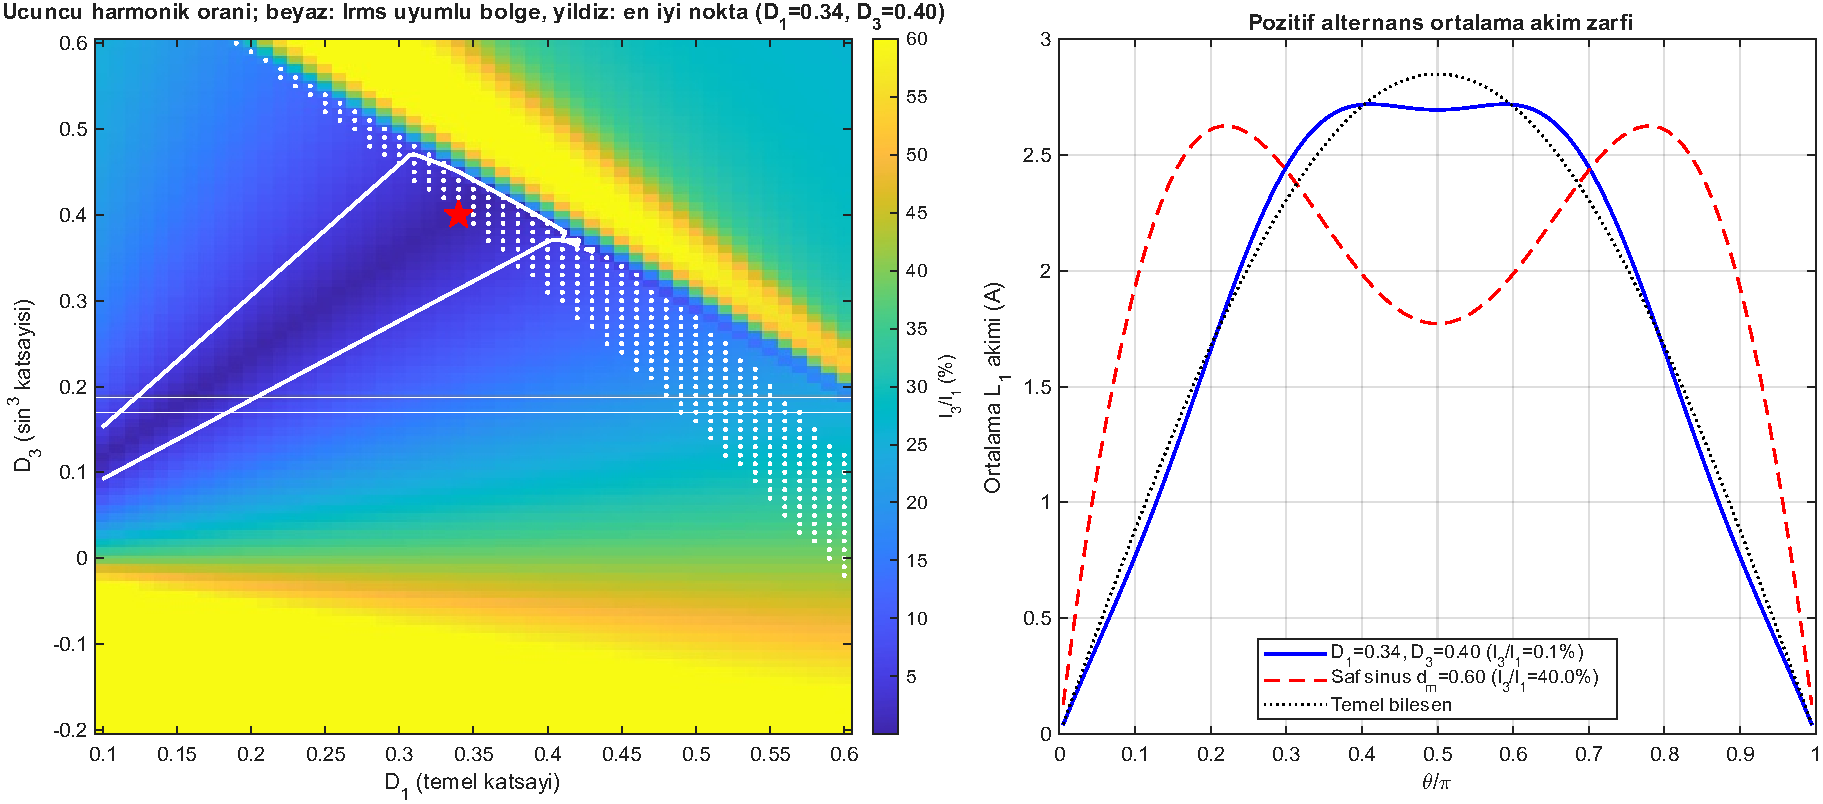
\includegraphics[width=\textwidth]{../tez-matlab-simulink/results/sin3_rescan_20260901/sin3_katsayi_taramasi_20260901.pdf}
  \caption{$(D_1,D_3)$ katsayı düzleminde üçüncü harmonik oranı (sol; beyaz noktalar \SI{2.0}{}--\SI{2.6}{\ampere} RMS bölgesini, yıldız en iyi noktayı gösterir) ve en iyi nokta ile saf sinüs görev oranının ortalama akım zarfı karşılaştırması (sağ). Parçalı DCM/CCM analitik modeli, 01.09.2026 hesabı.}
  \label{fig:sin3-yeniden-tarama}
\end{figure}

Eşitlik~\eqref{eq:sin3-duzeltilmis-optimum} ile verilen çift, uygulanan kazanç değil, tek endüktanslı analitik katmanın adayıdır. Anahtarlamalı benzetimde kullanılan S3 katsayıları ($K_{13}$, $K_{33}$) Alt Bölüm~\ref{sec:kalibrasyon} içinde deney özetinin aktif ve reaktif gücüne kalibre edilmiştir ve harmonik eşdeğerleri $(K_{13}+3K_{33}/4,\ -K_{33}/4)=(0{,}7317,\ -0{,}0961)$'dir. Üçüncü harmonik katsayıları iki katmanda birbirine yakındır ($-0{,}10$ ile $-0{,}096$); temel katsayıdaki fark ($0{,}64$ ile $0{,}73$), analitik modelin içermediği $C_f$--$L_2$ ağı, ölü zaman, kayıplar ve köprünün süreksiz iletimdeki yumuşak gerilim kaynağı davranışından (Alt Bölüm~\ref{sec:kalibrasyon}) kaynaklanır ve analitik adayın \SI{2.02}{\ampere}, kalibre noktanın \SI{2.28}{\ampere} RMS akımda tanımlı olduğu da göz önünde tutulmalıdır. İki katsayı takımının karşılaştırması bir doğrulama değil, analitik katmanın üçüncü harmonik ihtiyacını doğru büyüklükte öngördüğüne ilişkin bir tutarlılık gözlemidir.

\section{Önerilen Yapı ve İleri Besleme Mekanizması}

İleri besleme yolunun fiziksel işlevi, evirici tarafındaki eşdeğer kaynak gerilimini şebeke gerilimine yaklaştırmaktır. PLL şebekeye kilitlendikten sonra, akım komutu uygulanmadan önce, evirici çıkışı ile şebeke eşpotansiyel ise seri $Z_1+Z_2$ filtre ve şebeke empedansından akan akım sıfıra yaklaşır. Şekil~\ref{fig:espotansiyel}, eşpotansiyel durumu eşdeğer kaynaklar ve iki kaynağın eşit gerilim dalga biçimleri üzerinde göstermektedir. Akım referansı uygulandığında denetleyicinin üretmesi gereken ek gerilim yalnız empedans düşümünü karşılayan küçük bir bileşendir; akım küçüldükçe ek bileşen mutlak olarak küçülür ve modeldeki küçük gerilim hataları göreli olarak daha görünür hâle gelir. İleri besleme teriminin düşük akımdaki göreli önemi aynı mekanizmadan kaynaklanır.

\begin{figure}[H]
  \centering
  \resizebox{\textwidth}{!}{%
  \begin{tikzpicture}[font=\small, x=1mm, y=1mm,
    tel/.style={thick},
    emp/.style={draw, thick, fill=white, minimum width=12mm, minimum height=5mm, inner sep=1pt}]
    % eşdeğer devre
    \draw[tel] (0,0) -- (0,30) -- (60,30) -- (60,0) -- cycle;
    \node[emp] at (20,30) {$Z_1$};
    \node[emp] at (42,30) {$Z_2$};
    \draw[thick, fill=white] (0,15) circle (5); \draw (-2.5,15) sin (-1.25,16.5) cos (0,15) sin (1.25,13.5) cos (2.5,15);
    \draw[thick, fill=white] (60,15) circle (5); \draw (57.5,15) sin (58.75,16.5) cos (60,15) sin (61.25,13.5) cos (62.5,15);
    \node[left] at (-6,15) {$v_{\mathrm{inv}}$};
    \node[right] at (66,15) {$v_g$};
    \draw[-{Latex[length=2mm]}, thick, red!70!black] (28,34) -- node[above]{$i=(v_{\mathrm{inv}}-v_g)/(Z_1+Z_2)=0$} (36,34);
    \node[align=center, font=\footnotesize] at (30,-6) {evirici eşdeğer kaynağı \hspace{14mm} şebeke};
    % dalga biçimleri
    \begin{scope}[xshift=82mm, yshift=18mm]
      \draw[-{Latex[length=1.5mm]}] (0,0) -- (52,0) node[right]{$t$};
      \draw[-{Latex[length=1.5mm]}] (0,-13) -- (0,14) node[above]{$v$};
      \draw[very thick, blue!70!black] plot[domain=0:50, samples=80] (\x, {11*sin(9*\x)});
      \draw[thick, dashed, orange!90!black] plot[domain=0:50, samples=80] (\x, {11*sin(9*\x)});
      \node[font=\footnotesize, align=left, anchor=west] at (2,-17) {\textcolor{blue!70!black}{---} $v_{\mathrm{inv}}$ \quad \textcolor{orange!90!black}{-\,-} $v_g$};
    \end{scope}
    \begin{scope}[xshift=82mm, yshift=-12mm]
      \draw[-{Latex[length=1.5mm]}] (0,0) -- (52,0) node[right]{$t$};
      \draw[-{Latex[length=1.5mm]}] (0,-5) -- (0,6) node[above]{$i$};
      \draw[very thick, red!70!black] (0,0) -- (50,0);
      \node[font=\footnotesize, anchor=west] at (2,3) {$i=0$};
    \end{scope}
  \end{tikzpicture}%
  }
  \caption[Eşpotansiyel evirici ve şebeke kaynakları]{İleri beslemenin eşpotansiyel durumu: evirici eşdeğer kaynağı ile şebeke kaynağı aynı genlik ve fazda olduğunda seri $Z_1$ (filtre) ve $Z_2$ (şebeke) empedanslarından akım akmaz. Şekil, akım komutu öncesindeki başlangıç durumunun ideal çözümüdür; kapalı çevrim izleme başarımını göstermez.}
  \label{fig:espotansiyel}
\end{figure}

Denetleyicinin devre dışı bırakılıp yalnız ileri besleme katsayısının değiştirildiği benzetim koşulu, yöntemin açık çevrim mekanizmasını ayırmak için yararlıdır; ancak kapalı çevrim başarımı ya da kararlılık kanıtı değildir. Şebeke gerilimi ileri beslemesi ideal durumda evirici ile şebeke gerilimini yaklaştırarak düşük akımdaki göreli gerilim hatasını azaltabilir; LCL filtre, ortak bağlantı noktası ölçümü ve sayısal gecikme eklendiğinde aynı yol sanal empedans ve aktif sönümleme etkisi de oluşturabilir \citep{Lu2016}. İleri besleme yolunun etkisi yalnız gerilim düşümü hesabıyla sınırlandırılmamıştır. Sin\textsuperscript{3} yolunun modülasyon toplamındaki konumu Şekil~\ref{fig:denetim-modulasyon-blok} üzerinde verilmiştir.

\section{Senaryo~3 Benzetim Kayıtları}
\label{sec:sin3-senaryo3-kayitlari}

Şekil~\ref{fig:s3-kalibre-l1}, kalibre S3 modelinde $L_1$ akımını ve şebeke akımını gösterir. Sin\textsuperscript{3} terimi, S2'de alternans ortasında çöken şebeke akımı zarfını sinüse yaklaştırır; $L_1$ akımı susturmalı çalışmanın süreksiz iletim yapısını korur, ters akım aralığı yoktur ve pozitif yarım periyodun \%27,6'sında akım sıfırdadır. Kompanzasyon süreksiz iletimi ortadan kaldırmaz; darbe genişliklerini, süreksiz iletimin ürettiği üçüncü harmoniği karşılayacak biçimde değiştirir.

\begin{figure}[H]
  \centering
  \includegraphics[width=0.96\textwidth]{model_dogrulama/s3_kalibre_l1.pdf}
  \caption[Kalibre benzetimde S3 $L_1$ akımı]{Kalibre benzetimde S3 (susturma + Sin\textsuperscript{3}): (a) son tam şebeke periyodunda $i_{L1}$, şebeke akımı $i_g$ ve karşılaştırma için S2 şebeke akımı; (b) pozitif yarım periyottan \SI{400}{\micro\second} kesitte $i_{L1}$.}
  \label{fig:s3-kalibre-l1}
\end{figure}

Kalibre S3 modeli deneydeki \%14 akım THD'sini \%14,8 ile yeniden üretmektedir (Alt Bölüm~\ref{sec:kalibrasyon}). Deneyde susturma THD'yi \%15'ten \%47'ye çıkarmış, Sin\textsuperscript{3} terimi \%14'e indirmiştir; S3, klasik anahtarlamanın harmonik düzeyine dönerken verimi klasik anahtarlamadan 2,0 puan yüksek tutmaktadır. Sonuç, Sin\textsuperscript{3} yolunun üçüncü harmonik cezasını önemli ölçüde azalttığını destekler. S1, S2 ve S3 deneylerinin DA bara gerilimleri (\SI{431.5}{}, \SI{395.0}{} ve \SI{427.5}{\volt}) ve şebeke gerilimleri (\SI{119.8}{}, \SI{121.0}{} ve \SI{124.3}{\volt}) birbirinden farklıdır (Tablo~\ref{tab:sistem-parametreleri}, Tablo~\ref{tab:deney-kosullari}). Her benzetim kendi deneyinin DA bara ve şebeke gerilimiyle yapılmıştır; deney ile benzetim aynı koşuldadır, ancak üç yöntem birbirinden farklı gerilimlerde çalıştığı için yöntemler arası karşılaştırma tek değişkenli değildir.

\section{Senaryo~4: Akım Geri Beslemeli Kapalı Çevrim}
\label{sec:s4-kapali-cevrim}

Senaryo~1--3 açık çevrim modülasyonla, deney donanımının yaklaşık \SI{2.3}{\ampere} faz akımında çalışmaktadır. Nötr susturma ve Sin\textsuperscript{3} ileri beslemesinin anma akımına taşınıp taşınamayacağı ve akım denetimiyle birlikte nasıl davrandığı Senaryo~4 (S4) ile incelenmiştir. S4, S3 modeline $L_1$ akımı geri beslemesi eklenerek kurulmuştur; güç katı ve ölçüm blokları S3 ile aynıdır (Şekil~\ref{fig:s3-simulink-modeli}), fark anahtarlama girişindedir (Şekil~\ref{fig:s4-anahtarlama-girisi}). Model çiziminde geri besleme oransal kazançla gösterilmiştir; tezdeki S4 benzetimlerinde denetleyici S3 tabanına betikle eklenmiş ve oransal denetleyiciye ek olarak PI ve PIR seçenekleriyle kurulmuştur (Alt Bölüm~\ref{sec:model-dogrulama-duzeltme}).

\begin{figure}[H]
  \centering
  \includegraphics[width=0.82\textwidth]{umit_2026-11-09/s4_anahtarlama_girisi.pdf}
  \caption[S4 modelinin anahtarlama girişi]{S4 modelinin anahtarlama girişi: Sin\textsuperscript{3} ileri beslemesi ($K_{14}$, $K_{34}$), $L_1$ akımı geri beslemeli oransal denetleyici ($K_p$), doyum ve kapı mantığı alt sistemi (\textsc{anahtarlama}). Güç katı ve ölçüm blokları Şekil~\ref{fig:s3-simulink-modeli} ile aynıdır.}
  \label{fig:s4-anahtarlama-girisi}
\end{figure} S4 için donanım deneyi yoktur; Alt Bölüm~\ref{sec:s4-kapali-cevrim} içindeki bütün sayılar benzetim sonucudur ve kalibre S3 modelinin kapalı çevrimle anma akımına taşınmasını gösterir.

\subsection{Model ve denetleyici yapısı}

S4 modülasyon komutu, ileri besleme ve geri besleme terimlerinin doyumlu toplamıdır:
\begin{equation}
  \begin{gathered}
    u=\operatorname{sat}_{\pm1}\!\left(u_{\mathrm{ff}}+u_{\mathrm{fb}}\right),\qquad
    u_{\mathrm{ff}}=K_{14}\sin(\theta+\varphi_4)+K_{34}\sin^3(\theta+\varphi_4),\\
    u_{\mathrm{fb}}=C(s)\left[i_{\mathrm{ref}}-H_m(s)\,i_{L1}\right],\qquad
    i_{\mathrm{ref}}=\sqrt2\,I_{\mathrm{ref}}\sin\theta .
  \end{gathered}
  \label{eq:s4-denetim-yapisi}
\end{equation}
Eşitlik~\eqref{eq:s4-denetim-yapisi} içinde $\theta$ şebekeye kilitli açı (ideal PLL), $H_m(s)$ tek kutuplu ölçüm süzgeci ve $C(s)$ akım denetleyicisidir. İleri besleme kazançları $K_{14}$, $K_{34}$ ve faz $\varphi_4$, kalibre S3 değerleridir (Tablo~\ref{tab:sistem-parametreleri}). Üç denetleyici aynı alt sistemde kazanç seçimiyle gerçeklenmiştir:
\begin{equation}
  C_{\mathrm{P}}(s)=K_p,\qquad
  C_{\mathrm{PI}}(s)=K_p+\frac{K_i}{s},\qquad
  C_{\mathrm{PIR}}(s)=C_{\mathrm{PI}}(s)+\frac{2K_r\omega_b s}{s^2+2\omega_b s+\omega_0^2}.
  \label{eq:s4-denetleyiciler}
\end{equation}
Oransal kazanç parametre dosyasındaki değerdir. PI sıfırı \SI{60}{\hertz}'e, yani birinci kazanç geçiş frekansının (yaklaşık \SI{586}{\hertz}, Tablo~\ref{tab:kararlilik-marjlar}) yaklaşık onda birine yerleştirilmiştir; \SI{60}{\hertz} değerinin şebeke frekansıyla ilgisi yoktur. Sıfırın geçiş frekansının onda birinde olması, integral teriminin geçişte getirdiği faz kaybını $\arctan(60/586)\simeq6^{\circ}$ ile sınırlar; P ve PI çevrimlerinin birinci geçişteki faz marjı farkı $5{,}9^{\circ}$'dir. PI denetleyicinin doyum önlemesi geri hesaplama yöntemiyle kurulmuştur. Kazançların tamamı Tablo~\ref{tab:sistem-parametreleri} içindeki S4 akım denetimi grubundadır. Denetim, modelde analog eşdeğeri olarak gerçeklenmiştir: denetleyici \SI{1}{\micro\second} adımla çalışır ve hesaplama gecikmesi yoktur. Analog eşdeğerin seçilme gerekçesi, PWM periyodu başında örnekleyip bir periyot gecikmeyle uygulayan sayısal gerçeklemenin LCL rezonansında kararsız olmasıdır; gerekçe Alt Bölüm~\ref{sec:kararlilik-bode} içinde sayısal olarak verilmektedir. $L_1$ doyumu modellenmemiştir.

\textbf{DA bara önkoşulu.} Faz başına modelde faz akımının tamamı bara kapasitörlerinden geçtiği için orta nokta salınımı akımla büyür (Alt Bölüm~\ref{sec:model-dogrulama-duzeltme}). Faz başına modelin bara kapasitörleri (2$\times$\SI{470}{\micro\farad}) üç fazlı deney donanımının toplam bara kapasitansından bir faza düşen paydır; üç fazlı donanımda toplam kapasitans faz payının üç katıdır. Faz payı kapasitansla modeldeki salınım \SI{2.3}{\ampere}'de yaklaşık \SI{11}{\volt} ($V_{\mathrm{dc}}/2$'nin \%5'i), \SI{25}{\ampere}'de ise yaklaşık \SI{120}{\volt} (\%56) olmaktadır. Faz payı kapasitansla yapılan PI benzetiminde evirici darbe yüksekliği pozitif alternans boyunca yaklaşık \SI{270}{\volt}'tan \SI{100}{\volt}'a inmiş, modülasyon zamanın \%20,6'sında doyuma girmiş ve kararlı durum oluşmamıştır: temel akım genlik hatası $-$\%31,9, THD \%57,4'tür. Orta nokta salınımı faz başına modelde \SI{25}{\ampere}'de büyüdüğü için S4 anma akımı benzetimlerinde bara kapasitansı 2$\times$\SI{5.6}{\milli\farad} değerine büyütülmüş ve salınım yaklaşık \SI{10}{\volt}'a (\%4,7) inmiştir (Tablo~\ref{tab:sistem-parametreleri}). Aynı PI denetleyicide genlik hatası $-$\%2,1'e, THD \%9,2'ye iner ve doyum ortadan kalkar. Anma akımında kapalı çevrim çalışmanın önkoşulu, DA bara orta noktasının tutulabilmesidir; büyütülmüş kapasitans değeri donanımda doğrulanmamıştır.

\subsection{Düşük, orta ve anma akımı taraması}

Tablo~\ref{tab:s4-tarama}, büyütülmüş DA bara ve kalibre ileri beslemeyle yapılan kesin taramayı vermektedir. Kararlı durum büyüklükleri son tam şebeke periyodundan alınmıştır; P ve PI benzetimleri \SI{0.06}{\second}, PIR benzetimleri rezonans teriminin dar bandı nedeniyle \SI{0.2}{\second} sürmüştür. Oturma ölçütü olarak son iki periyodun aktif güç farkı kullanılmış, tablodaki bütün benzetimlerde fark \%0,12'nin altında kalmıştır. Verim sütunu modelin DA ve AA güç ölçüm bloklarından alınmıştır. S4, $L_1$ çekirdek kaybı için S1--S3'ten farklı bir paralel direnç kullandığından (Tablo~\ref{tab:sistem-parametreleri}) S4 verimi yalnız S4 içinde karşılaştırılır; yaklaşık \SI{280}{\watt} çıkışta S4 verimi \%96,2, kalibre S3 verimi \%94,25'tir ve aradaki farkın yaklaşık \SI{7.2}{\watt}'lık kayıp karşılığı yalnız çekirdek kaybı parametresinden gelir.

\begin{table}[H]
  \centering
  \caption{S4 kapalı çevrim benzetimi: düşük, orta ve anma akımında akım izleme, harmonik, verim ve doyum (büyütülmüş DA bara, kalibre ileri besleme). PIR benzetimleri \SI{0.2}{\second}, diğerleri \SI{0.06}{\second}.}
  \label{tab:s4-tarama}
  \footnotesize
  \setlength{\tabcolsep}{2.6pt}
  \begin{tabular}{@{}l c c r r r r r c c@{}}
    \toprule
    Den., $I_{\mathrm{ref}}$ & $I_{L1,1}$ (A) & Genlik h. & Faz h. & THD$_I$ & $I_3/I_1$ & $P_{\mathrm{ac}}$ (W) & $\eta$ & Doyum & $|u|_{\max}$ \\
    \midrule
    P, \SI{2.3}{\ampere}   & 2,336 & $+$\%1,6  & $+1{,}0^{\circ}$ & \%7,0  & \%6,5  & 280,7 & \%96,24 & \%0 & 0,86 \\
    PI, \SI{2.3}{\ampere}  & 2,327 & $+$\%1,2  & $+1{,}4^{\circ}$ & \%7,2  & \%6,6  & 279,5 & \%96,20 & \%0 & 0,86 \\
    \midrule
    P, \SI{10}{\ampere}    & 7,677 & $-$\%23,2 & $-1{,}1^{\circ}$ & \%22,6 & \%20,9 & 922,5 & \%97,44 & \%0 & 0,87 \\
    PI, \SI{10}{\ampere}   & 8,918 & $-$\%10,8 & $-6{,}3^{\circ}$ & \%20,8 & \%18,7 & 1065  & \%97,31 & \%0 & 0,88 \\
    PIR, \SI{10}{\ampere}  & 9,777 & $-$\%2,2  & $+0{,}4^{\circ}$ & \%19,6 & \%18,7 & 1175  & \%97,28 & \%0 & 0,87 \\
    \midrule
    P, \SI{25}{\ampere}    & 22,15 & $-$\%11,4 & $-2{,}6^{\circ}$ & \%9,8  & \%9,6  & 2662  & \%96,69 & \%0 & 0,90 \\
    PI, \SI{25}{\ampere}   & 24,47 & $-$\%2,1  & $-4{,}0^{\circ}$ & \%9,2  & \%8,7  & 2938  & \%96,45 & \%0 & 0,90 \\
    PIR, \SI{25}{\ampere}  & 24,75 & $-$\%1,0  & $+0{,}2^{\circ}$ & \%8,5  & \%8,1  & 2978  & \%96,03 & \%0 & 0,93 \\
    \bottomrule
  \end{tabular}
\end{table}

\umitnot{İstenen THD sınırına ulaşıldı mı?}{Tezde şebeke standardıyla sayısal karşılaştırma yoktur; aşağıdaki hesap bilgi içindir. IEEE~1547 ve IEC~61727, toplam harmonik bozulmayı anma akımına göre (TDD) \%5, tek mertebeli 3--9. harmoniklerin her birini \%4 ile sınırlar. Anma akımı \SI{25}{\ampere} alınmıştır.
\begin{itemize}\setlength{\itemsep}{1pt}
  \item \textbf{\SI{2.3}{\ampere} (deney noktası): sınır içinde.} Harmonik akım anma akımının küçük bir kesridir. TDD: S1 yaklaşık \%1,3 (deneyin \%15'iyle; kalibre modelin \%39,5'iyle yaklaşık \%3,4), S2 yaklaşık \%4,0 (kalibre model \%4,8, sınıra yakın), S3 yaklaşık \%1,3. THD kendi temel bileşenine göre okunursa hiçbir senaryo \%5'e inmez; en iyisi S3, \%14.
  \item \textbf{\SI{10}{\ampere}: sınır dışı.} THD yaklaşık \%20, TDD yaklaşık \%7--8. Nedeni nötr susturmanın orta akımda çevrimin büyük kısmında süreksiz iletim yaratmasıdır.
  \item \textbf{\SI{25}{\ampere} (anma): sınır dışı.} THD PI ile \%9,2, PIR ile \%8,5; üçüncü harmonik \%8,7 ile tekil \%4 sınırını da aşar. Sin\textsuperscript{3} kazancı \SI{2.3}{\ampere}'e kalibre edildiğinden anma akımında üçüncü harmoniği artırır; terim kapatıldığında THD \%5,6'ya iner, yine sınırın biraz üstündedir.
  \item \textbf{Tezdeki yeri.} Orta akımda süreksiz iletim ve anma akımında ileri besleme genliği Bölüm~\ref{chap:sonuc} sınırlılıklarında (madde 5 ve 6) yazılıdır. Anma akımında sınırın altına inmek için akıma göre ayarlanan Sin\textsuperscript{3} genliği ya da susturmadan tamamlayıcı anahtarlamaya geçiş gerekir; ikisi de gelecek çalışma olarak önerilmiştir.
\end{itemize}}

Anma akımında PI ve PIR denetleyicileri referansı doyumsuz izlemektedir. PIR, \SI{50}{\hertz} rezonans terimiyle temel bileşen hatasını $-$\%1,0 ve $+0{,}2^{\circ}$'ye indirir; THD \%8,5, temel bileşen güç faktörü ($\cos\varphi_1$) 0,997'dir. Oransal denetleyici aynı noktada $-$\%11,4 genlik hatası bırakır; \SI{50}{\hertz}'teki sonlu çevrim kazancı kalıcı hatayı sıfırlamaz. Şekil~\ref{fig:s4-akim-izleme-25a}, \SI{25}{\ampere} noktasında üç denetleyicinin son iki şebeke periyodundaki $L_1$ akımını, referansı, çıkış akımını ve C noktası gerilimini birlikte göstermektedir; gerilim sağ eksende, şebeke nötrüne göre çizilmiştir. Şekil~\ref{fig:s4-tarama-ozet} ise verim, THD ve genlik hatasının akıma göre değişimini özetlemektedir.

\begin{figure}[H]
  \centering
  \includegraphics[width=\textwidth,height=0.62\textheight,keepaspectratio]{s4/s4_akim_izleme_25A_KC.pdf}
  \caption{S4 benzetiminde \SI{25}{\ampere} anma akımında P (üst), PI (orta) ve PIR (alt) denetleyicileriyle $L_1$ akımı (anlık ve anahtarlama periyodu ortalaması), akım referansı, çıkış akımı (sol eksen) ve şebeke nötrüne göre C noktası gerilimi $v_{ac}$ (sağ eksen, eksen sıfırları hizalı); son iki şebeke periyodu. Üç denetleyicide de $v_{ac}$'nin periyot ortalaması \SI{0.03}{\volt} altındadır.}
  \label{fig:s4-akim-izleme-25a}
\end{figure}

\begin{figure}[H]
  \centering
  \includegraphics[width=\textwidth]{s4/s4_tarama_ozet_KC.pdf}
  \caption{S4 benzetiminde verim, akım THD'si ($h\leq50$) ve temel bileşen genlik hatasının akım referansına göre değişimi; P, PI ve PIR denetleyicileri.}
  \label{fig:s4-tarama-ozet}
\end{figure}

\textbf{Orta akımda süreksiz iletim.} İzleme hatası akımla monoton değişmemektedir: \SI{10}{\ampere} noktası \SI{25}{\ampere} noktasından kötüdür. $L_1$ akım dalgalanması yaklaşık \SI{9}{\ampere} tepeden tepeye olduğundan anlık akımın mutlak değeri yaklaşık \SI{4.5}{\ampere}'in altına indiği her bölgede nötr susturmalı köprü süreksiz iletime girer ve senkron olmayan buck gibi davranır (Alt Bölüm~\ref{sec:dusuk-akim-modelleme}). \SI{25}{\ampere}'de süreksiz bölge yalnız sıfır geçişleri çevresindedir; \SI{10}{\ampere}'de ise çevrimin büyük kısmını kaplar. \SI{10}{\ampere}'de üçüncü harmonik baskındır ($I_3/I_1$ \%19--21). Kalibre Sin\textsuperscript{3} terimi \SI{2.3}{\ampere} noktasındaki bozulmaya göre ayarlandığından, süreksiz iletim bölgesi akımla değiştiğinde aynı terim \SI{10}{\ampere} noktasına uymamaktadır. PI'nin integral terimi genlik hatasını $-$\%23'ten $-$\%11'e indirir; PIR temel bileşeni $-$\%2,2 ve $+0{,}4^{\circ}$ ile kapatır, ancak THD \%19,6'da kalır, çünkü rezonans terimi yalnız \SI{50}{\hertz}'te etkilidir ve üçüncü harmonik bozulması süreksiz iletimden gelmektedir. Kararlılık analizi (Alt Bölüm~\ref{sec:kararlilik-bode}), \SI{10}{\ampere}'deki genlik hatasının bir kararlılık sorunu değil, köprünün etkin kazancındaki düşüşten doğan bir izleme sorunu olduğunu göstermektedir. Nötr susturma bir düşük güç yöntemidir: orta ve anma akımında tamamlayıcı anahtarlamaya dönüş ya da akım düzeyine göre ayarlanan ileri besleme gerekir. Kip geçişi tezin kapsamı dışındadır ve Bölüm~\ref{chap:sonuc} içinde öneri olarak yer almaktadır.

\subsection{Basamak yanıtı}

PI denetleyiciyle akım referansı $t=\SI{55}{\milli\second}$ anında \SI{10}{\ampere}'den \SI{25}{\ampere}'e basamak olarak değiştirilmiştir. Tablo~\ref{tab:s4-basamak} sonuçları vermektedir. Aşım, $L_1$ akım zarfının basamak sonrasındaki en büyük tepesinin son kararlı zarfa oranı olarak tanımlanmıştır. Kararlı durumda bile $L_1$ akımının tepesi, Sin\textsuperscript{3} kaynaklı üçüncü harmonik nedeniyle referans tepesinden \%7,3 yüksektir; aşım referans tepesine göre tanımlansaydı kararlı durumdaki dalga biçimi aşım gibi sayılırdı. Basamak sonrası kararlı değer, doğrudan \SI{25}{\ampere}'de başlatılan PI benzetimiyle aynıdır (\SI{24.48}{\ampere} ve \SI{24.47}{\ampere}); çözüm başlangıç koşulundan bağımsızdır. Basamak süresince geçici bileşenin sönümü Şekil~\ref{fig:s4-basamak} üzerinde, $K_{34}$ açık ve kapalı karşılaştırması ise Alt Bölüm~\ref{sec:kararlilik-bode} içinde verilmektedir.

\begin{table}[H]
  \centering
  \caption{S4 benzetiminde PI denetleyiciyle \SI{10}{\ampere}$\rightarrow$\SI{25}{\ampere} referans basamağı.}
  \label{tab:s4-basamak}
  \small
  \begin{tabularx}{0.9\textwidth}{@{}X r@{}}
    \toprule
    Büyüklük & Değer \\
    \midrule
    Basamak öncesi $I_{L1,1}$ (referans \SI{10}{\ampere}) & \SI{8.91}{\ampere} \\
    Basamak sonrası $I_{L1,1}$ (referans \SI{25}{\ampere}) & \SI{24.48}{\ampere} ($-$\%2,1) \\
    Aşım (son kararlı zarfa göre) & \%0,2 \\
    $L_1$ akım tepesinin referans tepesine oranı (kararlı durum, üçüncü harmonik dahil) & \%7,3 üstünde \\
    Yerleşme süresi (hata bandı) & \SI{0.44}{\milli\second} \\
    Geçişte doyum & zamanın \%0,8'i; $|u|_{\max}=1{,}49$ \\
    Basamak sonrası THD$_I$ & \%9,1 \\
    \bottomrule
  \end{tabularx}
\end{table}

\begin{figure}[H]
  \centering
  \includegraphics[width=\textwidth,height=0.5\textheight,keepaspectratio]{s4/s4_basamak_PI_10_25A_KC.pdf}
  \caption{S4 benzetiminde PI denetleyiciyle \SI{10}{\ampere}$\rightarrow$\SI{25}{\ampere} akım referansı basamağı: $L_1$ akımı, anahtarlama periyodu ortalaması ve modülasyon komutu.}
  \label{fig:s4-basamak}
\end{figure}

\section{Kararlılık ve Bode Analizi}
\label{sec:kararlilik-bode}

Sin\textsuperscript{3} yönteminin kapalı çevrim kararlılığı üç katmanda incelenmiştir. Birinci katman, Sin\textsuperscript{3} teriminin karakteristik denklemde yer almadığını analitik olarak gösterir. İkinci katman, S4 akım çevriminin açık çevrim kazancı $L$, duyarlılık fonksiyonu $S$ ve tamamlayıcı duyarlılık fonksiyonu $T$ için Bode eğrilerini, kazanç ve faz marjlarını ve kapalı çevrim kutuplarını $K_{34}$ açık ve kapalı hesaplar. Üçüncü katman, anahtarlamalı S4 modelinde küçük işaret enjeksiyonuyla ölçülen çevrim kazancını ve basamak yanıtını ortalama modelle karşılaştırır. Bütün sonuçlar benzetim modelinin kendi içindeki kararlılık kanıtıdır; S4 için donanım deneyi yoktur.

\subsection{Analitik katman: Sin\texorpdfstring{\textsuperscript{3}}{3} terimi çevrimin dışındadır}

Denetlenen sistem $G(s)=i_{L1}/v_{\mathrm{inv}}$, evirici kutup geriliminden $L_1$ akımına ortalama aktarım fonksiyonudur ve güç ağı anahtarlamalı modeldeki sırayla kurulmuştur: $L_1$ ve çekirdek kaybı direnci, $C_f$, EMC süzgecinin diferansiyel kip endüktansları ve X kapasitörü, $L_2$ ve şebeke (Tablo~\ref{tab:sistem-parametreleri}). Antirezonans (anti-resonance), LCL filtrede evirici geriliminden evirici tarafı ($L_1$) akımına giden yolun kazancının çöktüğü frekanstır; $C_f$ ile $L_2$'nin paralel rezonansına karşılık gelir ve yaklaşık $f_{\mathrm{antirez}}\simeq1/(2\pi\sqrt{L_2C_f})$ ile verilir. Ortalama modeldeki denetlenen sistemin rezonansı \SI{2815}{\hertz} ($\zeta=0{,}0041$), antirezonansı \SI{1720}{\hertz}'tir; antirezonans, $C_f$'ye EMC süzgecinin X kapasitörü eklendiği için yaklaşık ifadenin verdiği \SI{1.78}{\kilo\hertz}'in biraz altındadır. Normalize modülasyon komutunu kutup gerilimine dönüştüren PWM kazancı $K_{\mathrm{pwm}}=V_{\mathrm{dc}}/2$, toplam gecikme $T_d$ ve şebeke geriliminden akıma aktarım $G_g(s)$ ile gösterilsin. Açık çevrim (çevrim) kazancı $L$, çevrim bir noktadan açıldığında işaretin çevrimi bir kez dolaşırken uğradığı toplam kazançtır. Duyarlılık fonksiyonu $S=1/(1+L)$, bozucuların ve izleme hatasının çevrimce ne ölçüde bastırıldığını; tamamlayıcı duyarlılık fonksiyonu $T=L/(1+L)$ ise referansın çıkışa ne ölçüde aktarıldığını gösterir. $|S|\ll1$ olan frekanslarda bozucu bastırılır, $|T|\simeq1$ olan frekanslarda referans izlenir. Doyum dışında Eşitlik~\eqref{eq:s4-denetim-yapisi} çevrimi
\begin{equation}
  L(s)=C(s)\,K_{\mathrm{pwm}}\,e^{-sT_d}\,G(s)\,H_m(s)
  \label{eq:sin3-acik-cevrim}
\end{equation}
açık çevrim kazancını tanımlar. Duyarlılık ve tamamlayıcı duyarlılık fonksiyonları
\begin{equation}
  S(s)=\frac{1}{1+L(s)},
  \qquad
  T(s)=\frac{L(s)}{1+L(s)}
  \label{eq:sin3-duyarlilik}
\end{equation}
biçimindedir. Kapalı çevrimde $L_1$ akımı
\begin{equation}
  i_{L1}=\frac{K_{\mathrm{pwm}}e^{-sT_d}G(s)\left[u_{\mathrm{ff}}+C(s)\,i_{\mathrm{ref}}\right]+G_g(s)\,v_g}{1+L(s)}
  \label{eq:sin3-kapali-cevrim-girisleri}
\end{equation}
olarak yazılır. $\theta$ yalnız zamana bağlıdır ve şebekeye kilitlidir; $\sin^3\theta$ işaretinin hiçbir girişi çevrimdeki bir büyüklükten gelmez. Eşitlik~\eqref{eq:sin3-kapali-cevrim-girisleri} içinde $u_{\mathrm{ff}}$ yalnız payda, dış bir giriş olarak yer alır; karakteristik denklem $1+L(s)=0$, $K_{34}$'ü içermez. Kapalı çevrim kutupları, kazanç ve faz marjları $K_{34}$'ten bağımsızdır; $K_{34}$ yalnız dış girişin genliğini değiştirir. Doyum sınırı bütün kararlı durum pencerelerinde aşılmamıştır ($|u|_{\max}\leq0{,}93$, Tablo~\ref{tab:s4-tarama}); doyumsuz çalışmada doğrusal ayrım çalışma noktalarında geçerlidir.

Sin\textsuperscript{3} teriminin akıma etkisi $S(j\omega)K_{\mathrm{pwm}}G(j\omega)$ ile belirlenir. Eşitlik~\eqref{eq:sin3-esdeger-katsayilar} ile kalibre ileri besleme $0{,}7317\sin(\theta+\varphi_4)-0{,}0961\sin(3\theta+3\varphi_4)$ biçimindedir. PI denetleyicide $|S(j2\pi\cdot\SI{150}{\hertz})|=0{,}234$ ($-12{,}6$~dB) olduğundan, üçüncü harmonik modülasyonun çevrimsiz durumda üreteceği \SI{9.53}{\ampere} RMS \SI{150}{\hertz} akımı çevrim \SI{2.23}{\ampere} RMS'ye indirir; P ve PIR için oran 0,231 ve 0,214'tür. Temel bileşende Sin\textsuperscript{3}'ün payı ($3K_{34}/4$), ortalama modelde PI ile $L_1$ temel akımını \SI{22.71}{\ampere}'den \SI{25.18}{\ampere} RMS'ye taşır. Kapalı çevrimde ileri besleme, denetleyicinin karşılaması gereken temel bileşeni azaltır ve çevrim açısından bilinen bir dış giriştir; çevrimin kendisi, yani $L$, $S$ ve $T$, değişmez.

\subsection{Frekans alanı: marjlar, Bode eğrileri ve kutuplar}

Gerçekleme (A), modeldeki analog eşdeğerdir: sürekli denetleyici, \SI{5}{\kilo\hertz} ölçüm süzgeci ve üst sınır olarak $T_d=\SI{2}{\micro\second}$ toplam gecikme. Aynı yapının \SI{1}{\micro\second} ayrık karşılığı marjları en çok $0{,}02^{\circ}$ ve \SI{0.1}{\decibel} değiştirdiğinden ayrıca tablolanmamıştır. Gerçekleme (B) sayısal bir denetleyiciyi temsil eder: denetim periyodu bir PWM periyodu ($T_s=\SI{100}{\micro\second}$), periyot ortalamalı örnekleme, bir periyotluk hesaplama gecikmesi ve sıfırıncı mertebe tutucu. (B2), aynı yapının periyotta iki güncellemeli ($T_s=\SI{50}{\micro\second}$) biçimidir.

Denetlenen sistemdeki LCL filtre nedeniyle $|L(j\omega)|$ eğrisi 0~dB eksenini üç kez keser: birinci geçişten sonra antirezonansta düşen kazanç, rezonansa doğru yeniden yükselir ve rezonans tepesinden sonra tekrar düşer. Tek bir kesişim frekansıyla verilen marj tanımı eksik kalır. Tezde faz marjı her kazanç geçişi $f_i$ için ayrı hesaplanmıştır: $\mathrm{PM}_i=180^{\circ}-|\angle L(j2\pi f_i)|$; gecikme marjı $\mathrm{DM}_i$, $-1$ noktasına ulaşmak için gereken ek saf gecikmedir. Kazanç marjı, $L$'nin negatif gerçel ekseni kestiği faz geçişinde $\mathrm{GM}=-20\log_{10}|L|$ olarak tanımlanmıştır. LCL rezonansında $L$'nin fazı $0^{\circ}$'dan geçer ve $|L|\simeq\SI{30}{\decibel}$'dir; nokta pozitif gerçel eksendedir ve faz geçişi değildir. Kararlılık hükmü Nyquist ölçütüne dayanır: açık çevrimde kararsız kutup bulunmadığından ($P=0$), $(-\infty,-1)$ ışınının net kesişim sayısı sıfır olmalıdır. Ek olarak kapalı çevrim kutupları doğrudan hesaplanmış ve modül marjı $1/\|S\|_\infty$ verilmiştir. Üç ölçüt her satırda aynı sonucu vermektedir.

\begin{table}[H]
  \centering
  \caption{S4 akım çevriminin marjları (\SI{25}{\ampere}, ortalama model). Nyquist sütunu $(-\infty,-1)$ ışınının net kesişim sayısıdır; 0 kararlı, 1 kararsız. Bütün değerler $K_{34}$ açık ve $K_{34}=0$ için bit düzeyinde aynıdır.}
  \label{tab:kararlilik-marjlar}
  \scriptsize
  \setlength{\tabcolsep}{2.8pt}
  \begin{tabular}{@{}l l c c c r r c c@{}}
    \toprule
    Gerç. & Den. & Kazanç geçişleri (Hz) & $\mathrm{PM}_i$ ($^{\circ}$) & $\mathrm{DM}_{\min}$ (\si{\micro\second}) & Faz geçişi (Hz) & GM (dB) & $\|S\|_\infty$ (dB) & Nyquist \\
    \midrule
    A  & P   & 583 / 2454 / 3386 & 83,6 / 119,4 / 55,2 & 45,3 & 22\,167 & $+$35,3 & 2,28 & 0 \\
    A  & PI  & 586 / 2454 / 3386 & 77,7 / 120,8 / 54,2 & 44,4 & 22\,029 & $+$35,2 & 2,36 & 0 \\
    A  & PIR & 590 / 2454 / 3386 & 73,8 / 121,7 / 53,5 & 43,9 & 21\,937 & $+$35,2 & 2,42 & 0 \\
    \midrule
    B  & P   & 581 / 2474 / 3254 & 48,8 / 90,2 / 142,1 & 101 & 2811 & $-$30,3 & 5,12 & 1 \\
    B  & PI  & 574 / 2479 / 3246 & 43,3 / 88,7 / 142,1 & 99  & 2811 & $-$30,1 & 5,57 & 1 \\
    B  & PIR & 579 / 2479 / 3246 & 39,1 / 88,0 / 142,6 & 99  & 2810 & $-$30,0 & 6,02 & 1 \\
    B2 & PI  & 583 / 2440 / 3444 & 63,7 / 179,4 / 33,3 & 204 & 2863 & $-$20,4 & 4,97 & 1 \\
    \bottomrule
  \end{tabular}
\end{table}

Marj tablosunun satırları iki gerçeklemeyi, analog eşdeğer (A) ile sayısal (B ve B2) gerçeklemeyi, her gerçeklemede de P, PI ve PIR denetleyicilerini karşılaştırır; $K_{34}$ açık ve kapalı değerler bit düzeyinde aynı olduğundan ayrı satır açılmamıştır. Kazanç geçişleri sütunu $|L|=1$ olan frekansları, $\mathrm{PM}_i$ sütunu her geçişteki faz marjını, $\mathrm{DM}_{\min}$ sütunu çevrimin kararlılık sınırına ulaşmadan kaldırabileceği en küçük ek gecikmeyi, faz geçişi ve GM sütunları $\angle L=-180^{\circ}$ noktasındaki kazanç marjını, $\|S\|_\infty$ sütunu ise $L$ eğrisinin $-1$ noktasına en yakın uzaklığının tersini verir. Yaygın tasarım ölçütleri her kazanç geçişinde $\mathrm{PM}_i\gtrsim45^{\circ}$, $\mathrm{GM}\gtrsim\SI{6}{\decibel}$ ve $\|S\|_\infty\lesssim\SI{6}{\decibel}$'dir; $\mathrm{DM}_{\min}$ toplam denetim gecikmesinden büyük olmalıdır. Kesin kararlılık hükmü Nyquist sütunundadır (0 kararlı, 1 kararsız): negatif GM, faz geçişinde $|L|>1$ olduğunu ve $-1$ noktasının çevrelendiğini gösterir, kararsız satırlarda PM ve DM değerleri tek başına anlam taşımaz.

Tablo~\ref{tab:kararlilik-marjlar}, gerçekleme (A) için anma noktasındaki PI çevriminin kazanç geçişlerini \SI{586}{}, \SI{2454}{} ve \SI{3386}{\hertz}'te, faz marjlarını sırasıyla $77{,}7^{\circ}$, $120{,}8^{\circ}$ ve $54{,}2^{\circ}$ olarak vermektedir. Kritik faz marjı \SI{3.4}{\kilo\hertz}'teki $54^{\circ}$'dir; tek faz geçişi \SI{22}{\kilo\hertz}'tedir ve kazanç marjı $+$\SI{35}{\decibel}'dir (çevrim kazancı 57 katına kadar artabilir). Gecikme marjı \SI{44}{\micro\second}, $\|S\|_\infty$ \SI{2.4}{\decibel}'dir. Gerçekleme (A)'da faz rezonans çevresinde $+60^{\circ}$'den $-121^{\circ}$'ye iner ama $-180^{\circ}$'ye ulaşmaz, çünkü \SI{5}{\kilo\hertz} süzgeç ve \SI{2}{\micro\second} gecikme \SI{2.8}{\kilo\hertz}'te yalnız yaklaşık $31^{\circ}$ faz gecikmesi getirir; rezonans tepesi $-1$ noktasını çevrelemez. Şekil~\ref{fig:kararlilik-l-bode}, üç denetleyicinin $L$ Bode eğrilerini $K_{34}$ açık (çizgi) ve kapalı (işaretçi) olarak üst üste göstermektedir; eğriler örtüşmektedir. Şekil~\ref{fig:kararlilik-s-t}, $|S|$ ve $|T|$ eğrilerini \SI{50}{\hertz} ve \SI{150}{\hertz} işaretleriyle vermektedir.

\begin{figure}[H]
  \centering
  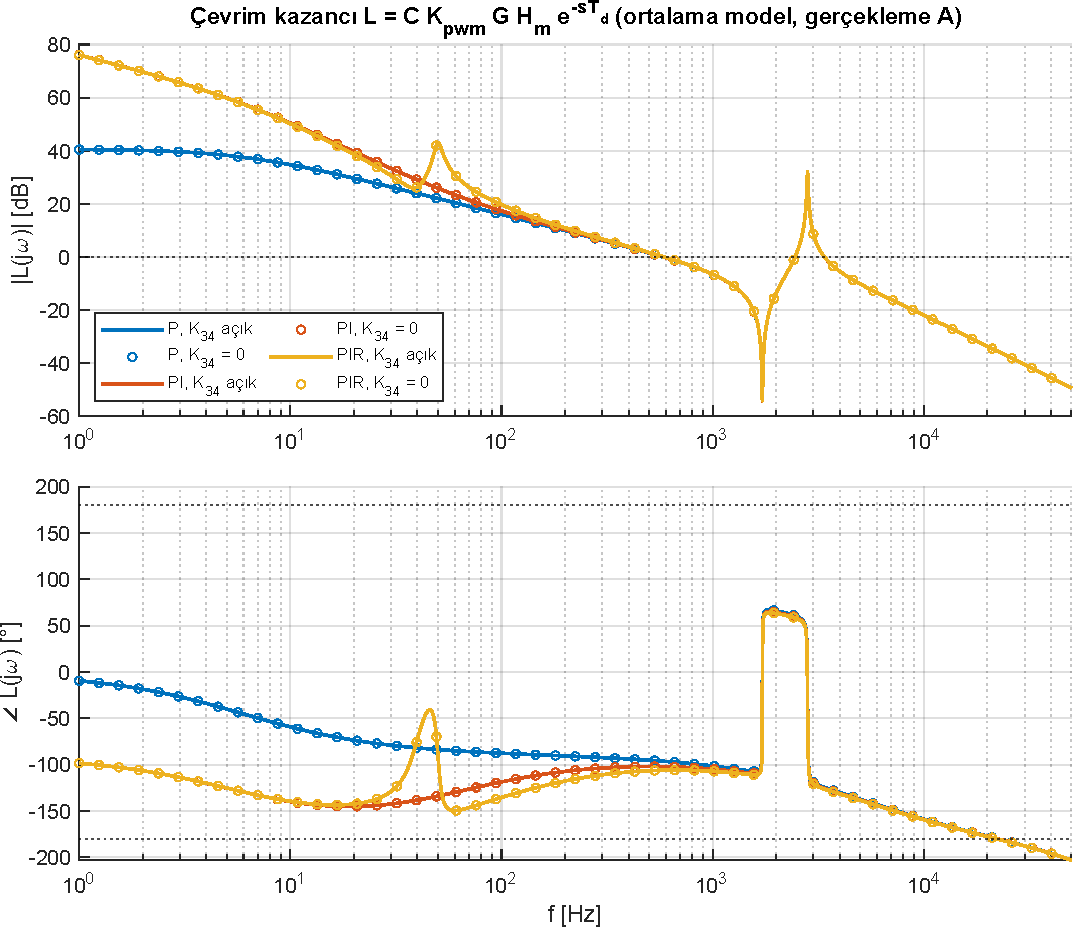
\includegraphics[width=\textwidth,height=0.5\textheight,keepaspectratio]{../tez-matlab-simulink/runs/2026-10-28_kararlilik/frekans/kararlilik_L_bode_K34.pdf}
  \caption{S4 akım çevriminin açık çevrim kazancı $L(j\omega)$, P, PI ve PIR denetleyicileri, gerçekleme (A), \SI{25}{\ampere}; $K_{34}$ açık (çizgi) ve $K_{34}=0$ (işaretçi) eğrileri örtüşür.}
  \label{fig:kararlilik-l-bode}
\end{figure}

\begin{figure}[H]
  \centering
  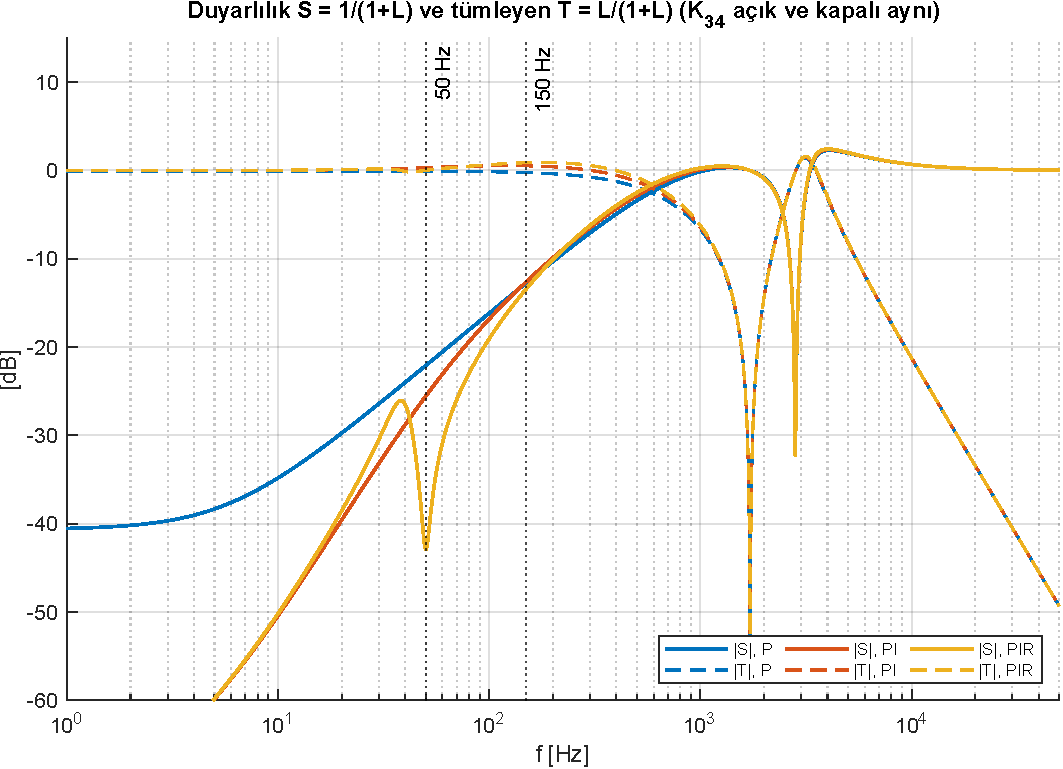
\includegraphics[width=\textwidth,height=0.45\textheight,keepaspectratio]{../tez-matlab-simulink/runs/2026-10-28_kararlilik/frekans/kararlilik_S_T.pdf}
  \caption{S4 akım çevriminin duyarlılık $|S(j\omega)|$ ve tamamlayıcı duyarlılık $|T(j\omega)|$ eğrileri; \SI{50}{\hertz} ve \SI{150}{\hertz} noktaları işaretlidir.}
  \label{fig:kararlilik-s-t}
\end{figure}

Kapalı çevrim kutupları kararlılık hükmünü bağımsız olarak doğrulamaktadır. Gerçekleme (A)'da en az sönümlü kutup çifti P için \SI{3097}{\hertz} ($\zeta=0{,}184$), PI için \SI{3109}{\hertz} ($\zeta=0{,}181$), PIR için \SI{3117}{\hertz} ($\zeta=0{,}179$) çevresindedir. PI'de PI sıfırına yakın \SI{66}{\hertz}'lik gerçel bir kutup, PIR'de ise rezonans teriminden gelen \SI{40.1}{\hertz}, $\zeta=0{,}155$ yavaş bir çift bulunur. Yavaş çiftin yaklaşık \SI{26}{\milli\second} zaman sabiti, PIR benzetimlerinin \SI{0.06}{\second}'de oturmayıp \SI{0.2}{\second} gerektirmesinin nedenidir.

Kararlılık sonucu, ortalama Simulink/Simscape modelinin Simulink Control Design ile doğrusallaştırılmasıyla ayrıca doğrulanmıştır. Ortalama modelde denetleyici alt sistemi, ölçüm süzgeci, doyum, doyum önleme ve ileri besleme blokları anahtarlamalı S4 modelindekilerle aynıdır; köprü, $K_{\mathrm{pwm}}$ kazançlı denetimli gerilim kaynağıyla temsil edilmiştir. Doğrusallaştırılan $L$ ile analitik $L$ arasındaki en büyük göreli fark P, PI ve PIR için sırasıyla $1{,}6\cdot10^{-11}$, $3{,}5\cdot10^{-10}$ ve $6{,}4\cdot10^{-4}$'tür (faz $\leq0{,}04^{\circ}$); $K_{34}$ açık ve kapalı doğrusallaştırmalar arasındaki fark sıfırdır.

\textbf{Sayısal gerçeklemenin kararsızlığı.} Gerçekleme (B)'de ortalama örnekleme, hesaplama ve tutucu gecikmelerinin toplamı iki PWM periyodudur (\SI{200}{\micro\second}) ve rezonansta fazı $-180^{\circ}$'nin altına iter. $L$, $|L|\simeq\SI{30}{\decibel}$ iken negatif gerçel ekseni $-32{,}7$ noktasında keser; Nyquist net kesişimi 1'dir ve \SI{2.72}{\kilo\hertz}'te bir çift kararsız kutup oluşur ($|z|=1{,}175$--$1{,}179$). Periyotta iki güncelleme (B2) de yetmez ($|z|=1{,}085$): gecikme \SI{100}{\micro\second}'ye inse de analog eşdeğerin \SI{44}{\micro\second}'lik gecikme marjının üstündedir. Gecikme taraması aynı sınırı doğrular: PI çevrimi $T_d=\SI{45}{\micro\second}$'de kararlı, \SI{50}{\micro\second}'de kararsızdır. Rezonans frekansı $f_s/6\simeq\SI{1.67}{\kilo\hertz}$'in üstünde olan LCL filtrede $L_1$ akımı geri beslemesi, sayısal gecikmeyle birlikte aktif sönümleme olmadan kararsızdır \citep{Lu2016,Wang2024}. S4, sayısal gerçeklemenin kararsızlığı göz önünde tutularak analog eşdeğer olarak sunulmuştur; sayısal gerçekleme için kapasitör akımı geri beslemesi gibi bir aktif sönümleme yöntemi ya da şebeke akımı geri beslemesi gereklidir. Şekil~\ref{fig:kararlilik-nyquist} iki gerçeklemenin Nyquist eğrilerini $-1$ noktası çevresinde göstermektedir. Gerçekleme (A)'da gecikme 0--\SI{10}{\micro\second} aralığında değiştirildiğinde en küçük faz marjı $56{,}6^{\circ}$'den $44{,}4^{\circ}$'ye iner; kararlılık hükmü değişmez.

\begin{figure}[H]
  \centering
  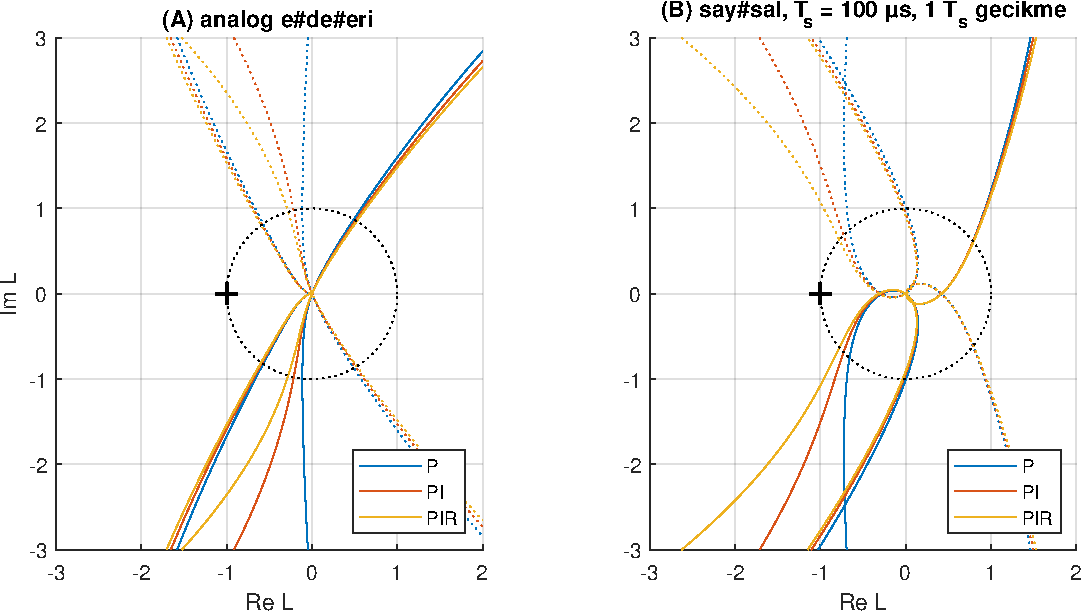
\includegraphics[width=\textwidth,height=0.45\textheight,keepaspectratio]{../tez-matlab-simulink/runs/2026-10-28_kararlilik/frekans/kararlilik_nyquist_A_B.pdf}
  \caption{S4 akım çevriminin Nyquist eğrileri: analog eşdeğer (A) $-1$ noktasını çevrelemez; bir periyot hesaplama gecikmeli sayısal gerçekleme (B) rezonansta negatif gerçel ekseni $-1$'in solunda keser.}
  \label{fig:kararlilik-nyquist}
\end{figure}

\textbf{Şebeke endüktansı duyarlılığı.} $L_2$, şebeke ve varyak endüktansını içerir. Zayıf şebeke ya da uzun hat etkisi için $L_2$'ye 0--\SI{5}{\milli\henry} ek endüktans $L_g$ eklenmiştir (Tablo~\ref{tab:kararlilik-lg}, Şekil~\ref{fig:kararlilik-lg}). Gerçekleme (A) bütün aralıkta kararlıdır; kritik geçişin faz marjı $54^{\circ}$'den $56^{\circ}$'ye hafifçe artar, kazanç marjı değişmez, çünkü yüksek frekansta $L$, $L_1$ ile belirlenir. Bedeli izleme bant genişliğidir: $L_g$ büyüdükçe antirezonans aşağı iner ve birinci geçiş \SI{586}{\hertz}'ten \SI{158}{\hertz}'e düşer. Gerçekleme (B) her $L_g$ değerinde kararsızdır ve kötüleşir.

\begin{table}[H]
  \centering
  \caption{Ek şebeke endüktansının S4 PI çevrimine etkisi.}
  \label{tab:kararlilik-lg}
  \small
  \begin{tabular}{@{}c c c c c c@{}}
    \toprule
    $L_g$ (mH) & $f_{\mathrm{res}}$ / $f_{\mathrm{antirez}}$ (Hz) & 1. geçiş (Hz) & $\mathrm{PM}_{\min}$ ($^{\circ}$) & GM (dB) & (B) $\max|z|$ \\
    \midrule
    0   & 2815 / 1720 & 586 & 54,2 & 35,2 & 1,175 \\
    0,5 & 2635 / 1406 & 450 & 54,9 & 35,2 & 1,215 \\
    1   & 2540 / 1218 & 367 & 55,3 & 35,2 & 1,236 \\
    2   & 2441 / 995  & 271 & 55,7 & 35,2 & 1,257 \\
    5   & 2337 / 704  & 158 & 56,1 & 35,2 & 1,277 \\
    \bottomrule
  \end{tabular}
\end{table}

\begin{figure}[H]
  \centering
  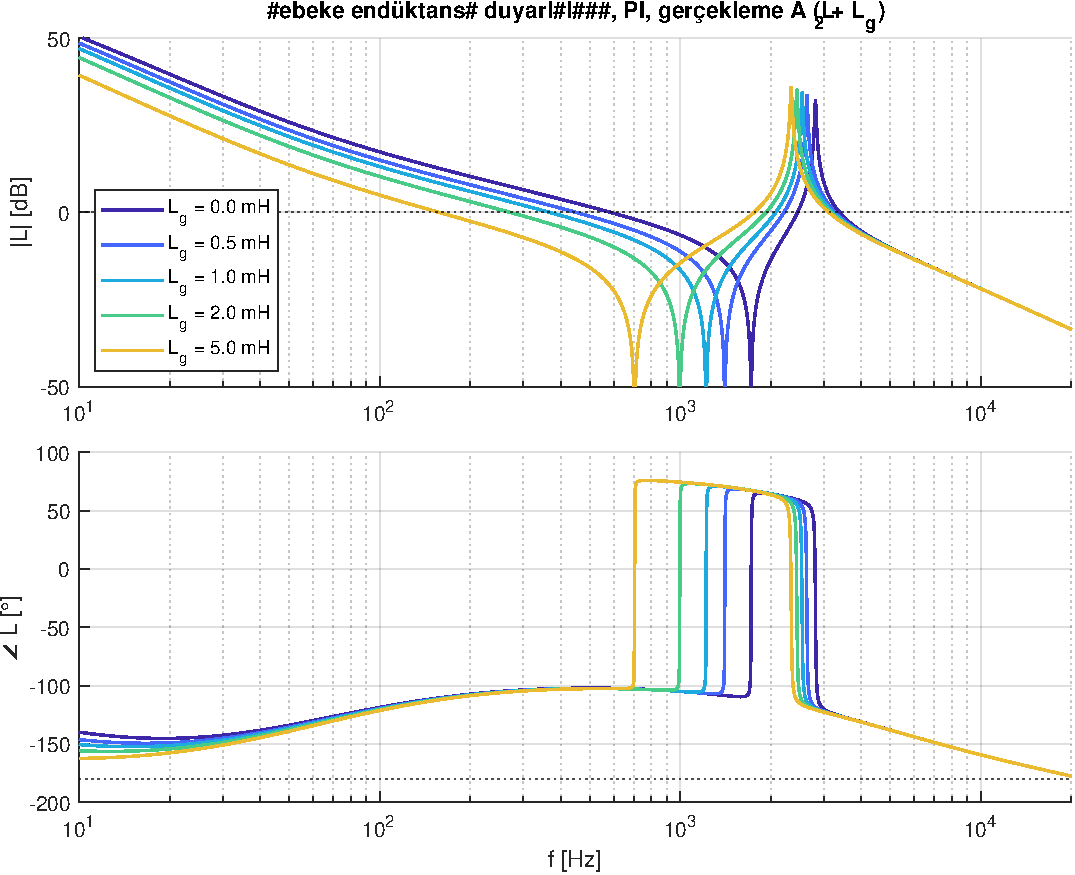
\includegraphics[width=\textwidth,height=0.42\textheight,keepaspectratio]{../tez-matlab-simulink/runs/2026-10-28_kararlilik/frekans/kararlilik_Lg_taramasi.pdf}
  \caption{Ek şebeke endüktansı $L_g=0$--\SI{5}{\milli\henry} için S4 PI çevriminin $L(j\omega)$ eğrileri, gerçekleme (A).}
  \label{fig:kararlilik-lg}
\end{figure}

Köprünün etkin küçük işaret kazancı süreksiz iletimde değişir. PWM kazancı $\lambda K_{\mathrm{pwm}}$ ile ölçeklendiğinde çevrim $\lambda=0{,}05$--50 aralığında kararlı, $\lambda=60$'ta kararsızdır; sınır $+$\SI{35.2}{\decibel} kazanç marjıyla tutarlıdır. Kazanç azalması kararlılığı bozmaz, yalnız birinci geçişi aşağı çeker ($\lambda=0{,}1$'de \SI{79}{\hertz}) ve izleme hatasını büyütür.

\subsection{Zaman alanı: anahtarlamalı modelde doğrulama}

Anahtarlamalı model doğrudan doğrusallaştırılamaz: PWM karşılaştırıcısının ve kip mantığının yerel türevi hemen her yerde sıfırdır ve doğrusallaştırma denetlenen sistemin yolunu keser. Çevrim kazancı, doğrusallaştırma yerine enjeksiyonla ölçülmüştür. Anahtarlamalı S4 modelinin bir ölçüm kopyasında modülasyon toplamına küçük bir işaret $d$ eklenmiştir ($u_x=u_{\mathrm{fb}}+d$); $d=0$ iken model taramadaki modelle matematiksel olarak aynıdır. $d$, her biri 0,015 genlikli üç tonlu (Schroeder fazlı) bir toplamdır; \SI{80}{\milli\second} pencerede tonlar \SI{50}{\hertz} harmoniklerine ve \SI{100}{\hertz} dönüşüm ürünlerine dik seçilmiştir (212,5 / 525 / 1037,5~Hz ve 587,5 / 2025 / 3362,5~Hz). Çevrim kazancı $L=-U_{\mathrm{fb}}/U_x$ olarak kestirilmiştir. Belirsizlik, tona komşu ve ton taşımayan ızgara noktalarındaki $u_x$ düzeyinden, yani anahtarlama ve kip dönüşümü kaynaklı arka plandan hesaplanmıştır. Enjeksiyonlu benzetimlerin temel bileşeni enjeksiyonsuz benzetimlerle aynıdır (PI, \SI{25}{\ampere}: \SI{24.46}{\ampere} ve \SI{24.47}{\ampere}); enjeksiyon çalışma noktasını bozmamıştır.

\begin{table}[H]
  \centering
  \caption{S4 PI çevrim kazancı $L(j\omega)$: analitik gerçekleme (A) ile anahtarlamalı modelde enjeksiyonla ölçülen değerler; hücrelerde $|L|$ (dB) / $\angle L$ ($^{\circ}$).}
  \label{tab:kararlilik-olcum}
  \scriptsize
  \setlength{\tabcolsep}{3pt}
  \begin{tabular}{@{}r c c c c c c@{}}
    \toprule
    $f$ (Hz) & Analitik (A) & \SI{25}{\ampere}, $K_{34}$ açık & \SI{25}{\ampere}, $K_{34}=0$ & \SI{10}{\ampere} & \SI{2.3}{\ampere} & Belirsizlik \\
    \midrule
    212,5  & 9,74 / $-106{,}7^{\circ}$ & 9,90 / $-94{,}4^{\circ}$ & 10,19 / $-90{,}2^{\circ}$ & 8,36 / $-68{,}5^{\circ}$ & $-7{,}25$ / $-25{,}8^{\circ}$ & $\pm1{,}4$~dB / $\pm10^{\circ}$ \\
    525    & 1,11 / $-102{,}2^{\circ}$ & 1,29 / $-94{,}5^{\circ}$ & 1,31 / $-93{,}4^{\circ}$ & 0,66 / $-84{,}7^{\circ}$ & $-8{,}11$ / $-30{,}1^{\circ}$ & $\pm0{,}8$~dB / $\pm6^{\circ}$ \\
    587,5  & $-0{,}03$ / $-102{,}3^{\circ}$ & 0,18 / $-95{,}3^{\circ}$ & 0,32 / $-93{,}8^{\circ}$ & $-0{,}19$ / $-86{,}5^{\circ}$ & -- & $\pm0{,}6$~dB / $\pm4^{\circ}$ \\
    1037,5 & $-7{,}10$ / $-105{,}3^{\circ}$ & $-6{,}05$ / $-98{,}6^{\circ}$ & $-6{,}75$ / $-90{,}4^{\circ}$ & $-7{,}00$ / $-91{,}6^{\circ}$ & $-10{,}05$ / $-48{,}8^{\circ}$ & $\pm1{,}0$~dB / $\pm7^{\circ}$ \\
    2025   & $-12{,}67$ / $+63{,}9^{\circ}$ & $-11{,}00$ / $+60{,}5^{\circ}$ & $-10{,}08$ / $+54{,}4^{\circ}$ & $-10{,}62$ / $+49{,}1^{\circ}$ & -- & $\pm0{,}7$~dB / $\pm5^{\circ}$ \\
    3362,5 & 0,31 / $-125{,}6^{\circ}$ & 0,47 / $-126{,}7^{\circ}$ & 0,59 / $-122{,}5^{\circ}$ & 0,25 / $-114{,}9^{\circ}$ & -- & $\pm0{,}4$~dB / $\pm2{,}5^{\circ}$ \\
    \bottomrule
  \end{tabular}
\end{table}

Tablo~\ref{tab:kararlilik-olcum} ve Şekil~\ref{fig:kararlilik-olcum}, ölçülen ve analitik çevrim kazançlarını karşılaştırmaktadır. Ölçüm yönteminin kendisi iki yoldan denetlenmiştir: ölçülen denetleyici tasarım değerine 0,995--1,004 oranında ve $0{,}6^{\circ}$ içinde, ölçülen pasif ağ $I_{L1}/V_{\mathrm{inv}}$ analitik $G$'ye 0,987--1,028 oranında ve $3{,}4^{\circ}$ içinde eşittir. Ölçülen ve analitik $L$ arasındaki fark, köprünün etkin küçük işaret kazancından gelmektedir. Anma akımında ortalama model kritik bölgeyi doğru vermektedir: \SI{3362.5}{\hertz}'te fark $+$\SI{0.16}{\decibel} ve $-1{,}1^{\circ}$, ölçüm belirsizliği $\pm$\SI{0.4}{\decibel} ve $\pm2{,}5^{\circ}$'dir. Ölçümden kestirilen kritik faz marjı \SI{25}{\ampere}'de $K_{34}$ açıkken yaklaşık $53\pm3^{\circ}$, $K_{34}=0$ iken yaklaşık $57\pm3^{\circ}$, \SI{10}{\ampere}'de yaklaşık $65\pm2^{\circ}$'dir; analitik değer $54{,}2^{\circ}$'dir. \SI{212}{}--\SI{1037}{\hertz} aralığında anahtarlamalı model $7$--$12^{\circ}$ faz öndeliği göstermektedir; faz öndeliği sıfır geçişleri çevresindeki süreksiz iletim ve ölü zaman davranışından gelir ve marjı artırır. $K_{34}$ açık ve kapalı ölçümler arasındaki fark 0,02--\SI{0.9}{\decibel} ve $1$--$8^{\circ}$'dir; fark her noktada iki ölçümün birleşik belirsizliği içinde ya da sınırındadır ve iki benzetimin farklı akımda (\SI{24.5}{\ampere} ve \SI{21.9}{\ampere}) çalışmasından kaynaklanır.

\begin{figure}[H]
  \centering
  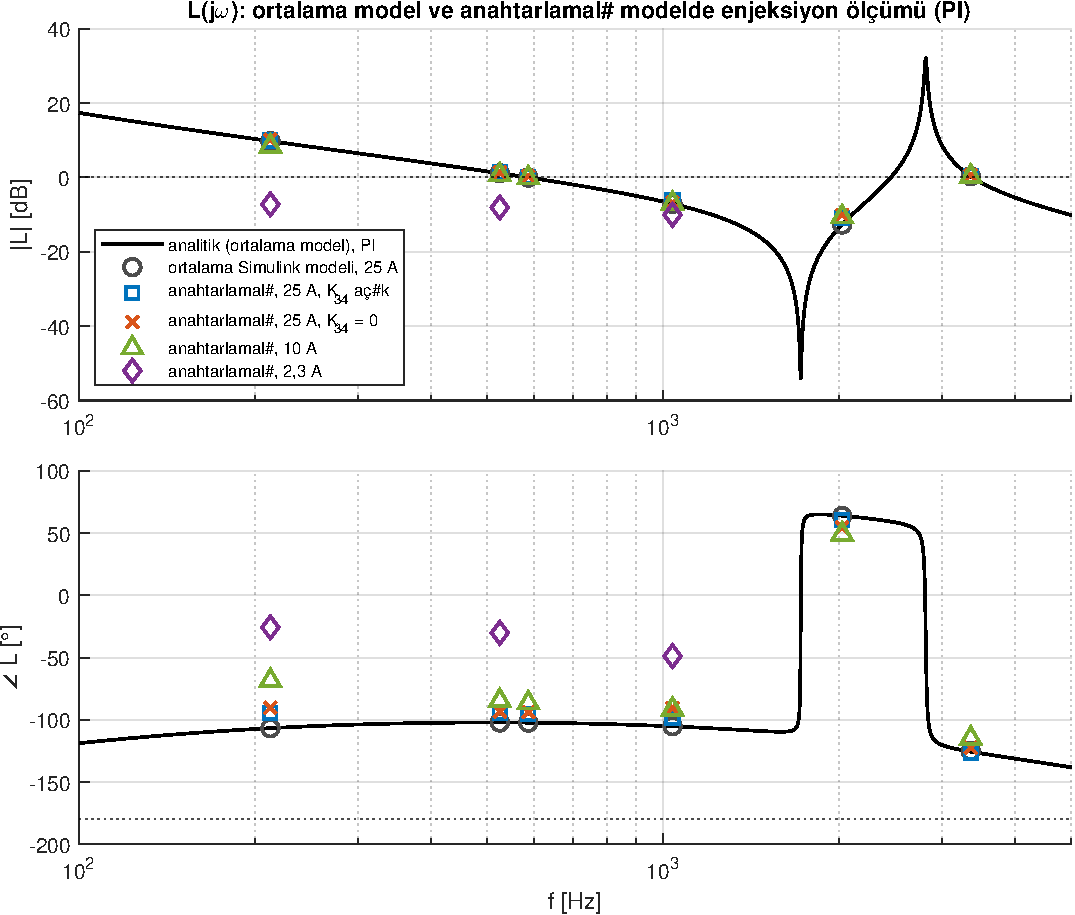
\includegraphics[width=\textwidth,height=0.45\textheight,keepaspectratio]{../tez-matlab-simulink/runs/2026-10-28_kararlilik/karsilastirma/kararlilik_L_olcum_karsilastirma.pdf}
  \caption{S4 PI çevrim kazancı: analitik $L(j\omega)$ eğrisi ile ortalama modelde ve anahtarlamalı modelde enjeksiyonla ölçülen noktalar (\SI{25}{\ampere} $K_{34}$ açık ve kapalı, \SI{10}{\ampere}, \SI{2.3}{\ampere}).}
  \label{fig:kararlilik-olcum}
\end{figure}

Orta ve düşük akımda köprünün etkin kazancı düşer ve faz öndeliği artar. \SI{10}{\ampere}'de etkin kazanç \SI{212}{\hertz}'te tasarım değerinin 0,87 katı ve $+40^{\circ}$ önde, \SI{2.3}{\ampere}'de ise 0,14--0,71 kat ve $+56$--$84^{\circ}$ öndedir. \SI{2.3}{\ampere}'de köprü süreksiz iletimde akım kaynağına yakın davranır: çevrim kazancı \SI{212}{}--\SI{1037}{\hertz} aralığında $-7$ ile \SI{-10}{\decibel} arasında, fazı $-49^{\circ}$'den öndedir; çevrim yavaş ama kararlıdır. Ortalama model düşük akımda izleme başarımını gerçekte olduğundan iyi gösterir; kararlılık sonucu ise korunur, çünkü ölçülen bütün noktalarda faz analitik değerden önde ya da ona eşittir ve köprü kazancının azalması kararlılığı bozmaz.

\textbf{Sin\textsuperscript{3}'ün üçüncü harmonik bulgusu.} Anma akımında $L_1$ akımındaki üçüncü harmoniğin kaynağı Sin\textsuperscript{3} teriminin kendisidir: \SI{25}{\ampere}'de $I_{L1,3}$, $K_{34}$ açıkken \SI{2.13}{\ampere}, $K_{34}=0$ iken \SI{0.43}{\ampere}'dir; THD sırasıyla \%9,4 ve \%5,6'dır. Kalibre $K_{34}$, \SI{2.3}{\ampere}'deki süreksiz iletim bozulmasını kompanze edecek büyüklüktedir; anma akımında bozulma küçük olduğundan terim fazla gelir ve çevrim onu $|S(j2\pi\cdot\SI{150}{\hertz})|=0{,}23$ oranında bastırır ama sıfırlamaz. Temel bileşende ise terim yararlıdır: $K_{34}=0$ iken PI genlik hatası $-$\%2,1'den $-$\%12,3'e çıkar. Kapalı çevrimde ileri besleme genliğinin akım düzeyine göre ayarlanması önerilir; öneri tezde uygulanmamıştır.

\textbf{Basamak yanıtı.} \SI{10}{\ampere}$\rightarrow$\SI{25}{\ampere} basamağı anahtarlamalı ve ortalama modelde $K_{34}$ açık ve kapalı olarak yinelenmiştir (Tablo~\ref{tab:kararlilik-basamak}, Şekil~\ref{fig:kararlilik-basamak}). Geçici bileşen, $i_{L1}(t)-i_{L1}(t+\SI{20}{\milli\second})$ farkı olarak tanımlanmıştır. Dört benzetimde de geçici bileşen aynı biçimde yaklaşık \SI{1}{\milli\second}'de söner; süre \SI{3.1}{\kilo\hertz}, $\zeta=0{,}18$ kutup çiftiyle ve 0,8--\SI{3}{\kilo\hertz} gerçel kutuplarla uyumludur ve ardından \SI{66}{\hertz}'lik PI kipi gelir. Anahtarlamalı modelde $K_{34}$ açık ve kapalı geçici bileşenler arasındaki fark \SI{0.61}{\ampere} RMS'dir (basamak tepesinin \%2,9'u).

\begin{table}[H]
  \centering
  \caption{S4 PI \SI{10}{\ampere}$\rightarrow$\SI{25}{\ampere} basamağında $K_{34}$ açık ve kapalı geçici yanıt.}
  \label{tab:kararlilik-basamak}
  \small
  \begin{tabularx}{\textwidth}{@{}X c c >{\raggedright\arraybackslash}p{0.34\textwidth}@{}}
    \toprule
    Benzetim & Zarf aşımı & Yerleşme (ms) & Ortalama modelden geçici fark (ilk \SI{15}{\milli\second}) \\
    \midrule
    Anahtarlamalı, $K_{34}$ açık & \%0,17 & 0,43 & \SI{0.38}{\ampere} RMS (\%1,8) \\
    Anahtarlamalı, $K_{34}=0$    & $-$\%0,5 & 0,69 & \SI{0.67}{\ampere} RMS (\%3,1) \\
    Ortalama, $K_{34}$ açık      & \%0,0 & 0,41 & -- \\
    Ortalama, $K_{34}=0$         & \%1,5 & 0,66 & -- \\
    \bottomrule
  \end{tabularx}
\end{table}

\begin{figure}[H]
  \centering
  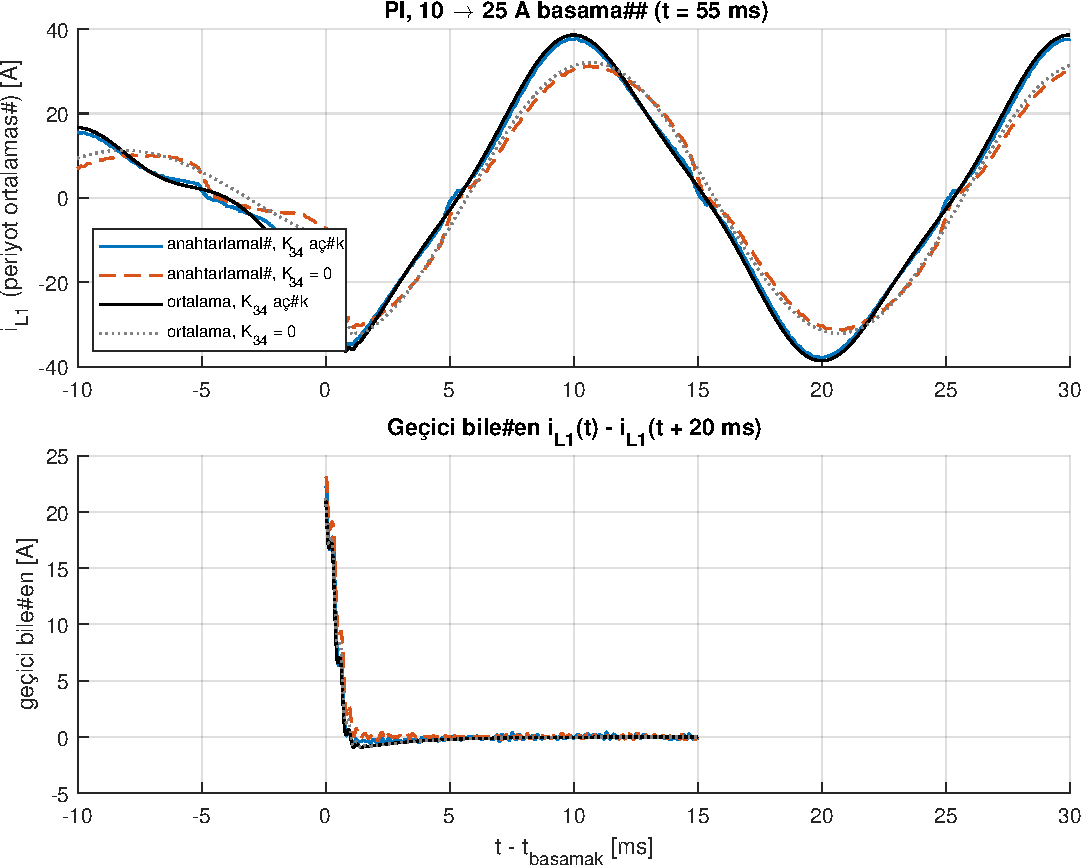
\includegraphics[width=\textwidth,height=0.45\textheight,keepaspectratio]{../tez-matlab-simulink/runs/2026-10-28_kararlilik/karsilastirma/kararlilik_basamak_K34.pdf}
  \caption{S4 PI \SI{10}{\ampere}$\rightarrow$\SI{25}{\ampere} basamağının geçici bileşeni; anahtarlamalı ve ortalama model, $K_{34}$ açık ve kapalı.}
  \label{fig:kararlilik-basamak}
\end{figure}

\subsection{Kararlılık analizinin sınırları}

Ortalama model, anma akımında sürekli iletim bölgesinde kritik frekans aralığını $\pm$\SI{0.2}{\decibel} ve $\pm1^{\circ}$ içinde vermektedir; orta ve düşük akımda köprünün etkin kazancı frekansa bağlı değiştiğinden ortalama model izleme başarımını iyimser gösterir. \SI{2.3}{\ampere}'de enjeksiyon ölçümü \SI{212}{}--\SI{1037}{\hertz} aralığını kapsar; 2--\SI{3.4}{\kilo\hertz} bölgesi ölçülmemiştir. Anahtarlamalı modelde enjeksiyon ölçümü PI denetleyiciyle yapılmıştır; denetlenen sistemin yanıtı ölçüldüğü ve denetleyicinin doğrusal olduğu doğrulandığı için P ve PIR çevrim kazançları ölçülen denetlenen sistem yanıtından yazılabilir. Gecikme $T_d=\SI{2}{\micro\second}$ bir üst sınırdır; analog eşdeğerin kararlılığı 0--\SI{10}{\micro\second} gecikme aralığında doğrulanmış ve gecikme marjı \SI{44}{\micro\second} bulunmuştur. Donanımın örnekleme yapısına ilişkin veri yoktur. Nötr susturmanın periyodik kip değişimi düşük akımda harmonikler arası bağlaşımı belirginleştirebilir; düşük akım için Eşitlik~\eqref{eq:htf-matris-iliskisi} çerçevesinde bir HTF ya da harmonik durum uzayı modeli kurulmamıştır \citep{Liao2022}. Faz payı bara kapasitansıyla \SI{25}{\ampere}'de kararlı durum oluşmadığından kararlılık analizi, S4 anma akımı benzetimlerindeki büyütülmüş bara kapasitansıyla yapılmıştır.

\section{Bölüm Sonucu}

Sin\textsuperscript{3} özdeşliği temel ve üçüncü harmonik bileşenini tek bir anlık terimde birleştirmekte, doğrudan $\sin(3\theta)$ enjeksiyonuyla aynı katsayı anlamını taşımamaktadır. Benzetim modelinde terim birim sinüsün küpü olarak, pozitif işaretle ve normalizasyonsuz biçimde modülasyon toplamına eklenmektedir. DCM/CCM parçalı modeli, nötr susturma sonrasında sinüzoidal görev oranının neden sinüzoidal akım üretmediğini göstermiş; doğru özdeşlikle yapılan analitik tarama, saf sinüs görev oranındaki \%39,96'lık üçüncü harmonik oranını $(D_1,D_3)=(0{,}34,\ 0{,}40)$ adayında \%0,15'e indirmiştir. Analitik adayın üçüncü harmonik katsayısı ($-0{,}10$), anahtarlamalı modelin kalibre katsayısına ($-0{,}096$) yakındır; katsayı seçimi çalışma noktasına bağlıdır.

S4 benzetiminde PI ve PIR akım denetimi \SI{25}{\ampere} anma akımında referansı sırasıyla $-$\%2,1 ve $-$\%1,0 genlik hatasıyla, doyumsuz ve \%8,5--9,2 THD ile izlemektedir; \SI{10}{\ampere}$\rightarrow$\SI{25}{\ampere} basamağında son kararlı zarfa göre aşım \%0,2, yerleşme \SI{0.44}{\milli\second}'dir. Anma akımı sonuçlarının önkoşulu, faz başına modelde DA bara orta noktasını tutabilen bir bara kapasitansıdır. Orta akımda (\SI{10}{\ampere}) nötr susturmanın yarattığı süreksiz iletim THD'yi \%20 düzeyine çıkarmakta ve yöntemin düşük güç kapsamını sınırlamaktadır.

Kararlılık analizi Sin\textsuperscript{3} teriminin bir denetleyici değil, çevrim dışından eklenen bilinen bir giriş olduğunu üç katmanda göstermiştir: karakteristik denklem $1+L(s)=0$ terimi içermez; $L$, $S$ ve $T$, $K_{34}$ açık ve kapalıyken ortalama modelde ve doğrusallaştırmada aynıdır, anahtarlamalı modelde ise farklar ölçüm belirsizliği düzeyindedir; terimin akıma etkisi $S(j\omega)K_{\mathrm{pwm}}G(j\omega)$ ile belirlenir ve \SI{150}{\hertz} bileşeni $|S|=0{,}23$ oranında bastırılır. Analog eşdeğer S4 çevrimi kritik geçişte $54^{\circ}$ faz marjı, $+$\SI{35}{\decibel} kazanç marjı ve \SI{44}{\micro\second} gecikme marjıyla kararlıdır ve 0--\SI{5}{\milli\henry} ek şebeke endüktansında kararlı kalır. Bir periyot gecikmeli sayısal gerçekleme ise aktif sönümleme olmadan kararsızdır; donanım uygulaması için aktif sönümleme gereklidir.
